\documentclass[letterpaper]{article}
\usepackage{aaai}
\usepackage{times}
\usepackage{helvet}
\usepackage{courier}
\usepackage{booktabs}
\usepackage{microtype}
\usepackage{amsmath}
\usepackage{amssymb}
\usepackage{graphicx}
\usepackage{float}
\usepackage{tikz}
\usepackage{fontawesome5}
\usetikzlibrary{arrows.meta,positioning,fit,backgrounds,calc,shapes.geometric}
\definecolor{panelA}{HTML}{EAF2EA}
\definecolor{panelB}{HTML}{EAF0FA}
\definecolor{boxedge}{HTML}{6B7280}
\definecolor{accentA}{HTML}{2E7D5B}
\definecolor{accentB}{HTML}{2F5BAA}
\definecolor{subcap}{HTML}{4B5563}
\frenchspacing
\setlength{\pdfpagewidth}{8.5in}
\setlength{\pdfpageheight}{11in}
\pdfinfo{
/Title (bioMoR: Biology-Prior-Guided Token Routing with Adaptive Recursive Computation for Genomic Learning)
/Author (Anonymous Submission)
/Keywords (single-cell genomics, multi-omics, transformers, parameter efficiency, marker genes, recursive computation, learned gene graph, calibration)
}
\setcounter{secnumdepth}{1}

\title{bioMoR: Biology-Prior-Guided Token Routing with Adaptive Recursive Computation for Genomic Learning}
\author{Anonymous Submission}

\begin{document}
\maketitle

\begin{abstract}
\begin{quote}
Genomic datasets often contain thousands of genes or pathways, making standard
transformers expensive because every token is processed through many independent layers.
Mixture-of-Recursions (MoR) reduces this cost through parameter sharing and adaptive token
depth, but allocates computation without using known biological relationships. We
introduce \textbf{bioMoR}, a biology-guided MoR framework for gene- and pathway-level
learning: it compresses the input into a small set of informative tokens, applies one
shared block recursively, and routes each token to an adaptive depth, while folding
gene--gene or pathway--pathway interaction structure into that routing to preserve
biologically relevant signals under a tight token and parameter budget. To our knowledge,
bioMoR is the first framework to integrate explicit biological interaction priors with
Mixture-of-Recursions for genomic modeling. Across eight single-cell datasets and three
multi-omics cancer cohorts (11 total), bioMoR improves mean macro-F1 over vanilla,
recursive, and biology-free MoR baselines and outperforms the vanilla transformer on most
datasets, under a unified 5-fold cross-validation protocol (all per-dataset figures are
reported with mean$\pm$SD over folds). Biological guidance thus improves the
accuracy--efficiency trade-off of recursive transformers for high-dimensional genomic data.
\end{quote}
\end{abstract}

\section{Introduction}
\label{sec:introduction}
\begin{figure*}[t]
\centering

\includegraphics[width=0.85\linewidth]{figs/overview.pdf}
\caption{\footnotesize\textbf{Overview of bioMoR.} Gene/pathway inputs are embedded and refined
by a shared \emph{biology prior} (gene--gene and pathway--pathway graphs); a selector
keeps the top-$M$ marker/pathway tokens; and a \emph{bio-router} combines a
data-driven and a biology-prior term to send only selected tokens through further
Mixture-of-Recursions steps (\emph{adaptive depth}). Pooled tokens feed a task head.
One pipeline serves single-cell and multi-omics data.}
\label{fig:overview}
\end{figure*}

\begin{table}[t]
\centering
\setlength{\tabcolsep}{3pt}
\resizebox{\linewidth}{!}{%
\begin{tabular}{lccccccc}
\toprule
& Pre- & Efficient & Multi- & Biology & Adaptive & Shared & Learned \\
Method & trained & tokens & omics & prior & depth & recursion & graph \\
\midrule
\multicolumn{8}{l}{\emph{Genomic / single-cell transformers}}\\
scGPT \cite{cui2024scgpt}                 & \checkmark & -- & -- & -- & -- & -- & -- \\
Geneformer \cite{theodoris2023transfer}   & \checkmark & -- & -- & -- & -- & -- & -- \\
scBERT \cite{scbert2022}                  & \checkmark & \checkmark & -- & -- & -- & -- & -- \\
scFoundation \cite{hao2024large}          & \checkmark & \checkmark & -- & -- & -- & -- & -- \\
UCE \cite{uce2026}                        & \checkmark & -- & -- & -- & -- & -- & -- \\
xTrimoGene \cite{xtrimogene2023}          & \checkmark & \checkmark & -- & -- & -- & -- & -- \\
tGPT \cite{tgpt2023}                      & \checkmark & -- & -- & -- & -- & -- & -- \\
scMulan \cite{scmulan2024}                & \checkmark & -- & -- & -- & -- & -- & -- \\
CellFM \cite{cellfm2025}                  & \checkmark & \checkmark & -- & -- & -- & -- & -- \\
LangCell \cite{langcell2024}              & \checkmark & -- & -- & -- & -- & -- & -- \\
Nicheformer \cite{nicheformer2024}        & \checkmark & -- & \checkmark & -- & -- & -- & -- \\
scRCL \cite{peng2026scrcl}                & \checkmark & -- & -- & -- & -- & -- & -- \\
GeneIncr.\ \cite{qi2026geneincremental}   & \checkmark & -- & -- & -- & -- & -- & -- \\
GeneMamba \cite{genemamba2024}            & \checkmark & \checkmark & -- & -- & -- & -- & -- \\
BMFM-RNA \cite{bmfmrna2025}               & \checkmark & -- & -- & -- & -- & -- & -- \\
CellPLM \cite{cellplm2024}                & \checkmark & -- & -- & \checkmark & -- & -- & -- \\
GeneCompass \cite{genecompass2024}        & \checkmark & -- & -- & \checkmark & -- & -- & -- \\
scMoFormer \cite{scmoformer2023}          & -- & -- & \checkmark & \checkmark & -- & -- & -- \\
GenoHoption \cite{cheng2024genohoption}   & \checkmark & -- & -- & \checkmark & -- & -- & -- \\
\addlinespace
\multicolumn{8}{l}{\emph{Adaptive-compute transformers}}\\
MoD \cite{raposo2024mixture}              & -- & -- & -- & -- & \checkmark & -- & -- \\
MoR \cite{bae2025mixture}                 & -- & -- & -- & -- & \checkmark & \checkmark & -- \\
\addlinespace
\multicolumn{8}{l}{\emph{Biology-structured models}}\\
genomap \cite{islam2023cartography}       & -- & -- & -- & \checkmark & -- & -- & -- \\
scTransformer \cite{sctransformer2024}    & -- & -- & -- & \checkmark & -- & -- & -- \\
DOGMA \cite{dogma2024}                    & -- & -- & \checkmark & \checkmark & -- & -- & -- \\
GATTACA \cite{mizera2026gattaca}          & -- & -- & -- & \checkmark & -- & -- & -- \\
P-NET/PATH \cite{elmarakeby2021biologically,howlader2026graph} & -- & \checkmark & \checkmark & \checkmark & -- & -- & -- \\
\midrule
\textbf{bioMoR (ours)}                    & -- & \checkmark & \checkmark & \checkmark & \checkmark & \checkmark & \checkmark \\
\bottomrule
\end{tabular}}
\caption{\footnotesize\textbf{Positioning of bioMoR against recent SOTA.} Columns are
the main contributions in this space -- large-scale \emph{pretraining}, \emph{efficient}
(sparse/compressed or sub-quadratic) token processing, \emph{multi-omics} inputs, a
structural \emph{biology prior}, per-token \emph{adaptive depth}, weight-\emph{shared
recursion}, and a \emph{learned} interaction graph. \checkmark{} = a built-in design
choice. Each method contributes along some axes; bioMoR is the only one that unifies a
biology prior and a learned graph with adaptive, weight-shared recursion (last four
columns), while also compressing tokens and handling multi-omics.}
\label{tab:positioning}
\end{table}

High-throughput sequencing produces increasingly large, high-dimensional molecular
datasets \cite{luecken2019current,hasin2017multiomics}: single-cell RNA sequencing
profiles each cell over more than 20,000 genes
\cite{luecken2019current,stuart2019integrative}, and multi-omics studies integrate
complementary layers such as genomic variation, transcriptomics, and epigenomics to
characterize disease \cite{hasin2017multiomics,stuart2019integrative}. Transformers
suit these data because self-attention learns dependencies among tokens
\cite{vaswani2017attention}, and models such as Geneformer, scBERT, scGPT, and
scFoundation show its promise for single-cell analysis and network biology
\cite{theodoris2023transfer,scbert2022,cui2024scgpt,hao2024large}. Yet transferring
the standard transformer to genomics creates a mismatch: all genes are treated as
tokens of equal computational status, although only a subset is informative for a
given cell type, cancer subtype, or task.

This mismatch is costly. Self-attention over $N$ tokens scales as $\mathcal{O}(N^2)$
\cite{vaswani2017attention}, so processing thousands of genes is expensive, and
stacking $K$ independent blocks makes the parameter count grow linearly with depth.
Efficient-attention methods such as Linformer, Performer, and Nystr\"omformer lower
the attention cost \cite{wang2020linformer,choromanski2021performer,xiong2021nystromformer}
but still spend equal computation on every gene, ignoring that genes and pathways
differ in predictive and biological importance.

Recursive and conditional-computation transformers target these costs. Universal
Transformers and ALBERT reuse one block across depth
\cite{dehghani2019universal,lan2020albert}; adaptive computation time,
mixture-of-experts, and Mixture-of-Depths allocate computation per input
\cite{graves2016act,shazeer2017moe,raposo2024mixture}; and, most related to us,
Mixture-of-Recursions (MoR) shares parameters across recursive steps while a
lightweight router gives each token its own recursion depth \cite{bae2025mixture}.
MoR's routing, however, is biology-agnostic: token depth is set from learned token
representations alone. For genomic data this is a real weakness -- a data-driven
router may stop a biologically important but weakly expressed gene too early, or
repeatedly process a prominent but redundant one, because it cannot see which genes
are functionally related.

Biology offers a natural remedy. Cell identities are defined by small marker-gene
sets \cite{aran2019singler,cortal2021cellid,ianevski2022sctype,franzen2019panglaodb,hu2023cellmarker},
and genes act through regulatory and signaling networks organized in resources like
Reactome \cite{gillespie2022reactome}. Existing biology-informed models -- P-NET,
genomap, and GenoHoption -- use such structure to constrain connectivity or
interpret representations
\cite{elmarakeby2021biologically,islam2023cartography,cheng2024genohoption}, but
not to decide how much computation each token receives. We therefore introduce a
\emph{bio-router} that folds a gene--gene or pathway--pathway graph directly into
the recursion-depth decision. Because curated graphs are incomplete and
context-dependent, we do not fix the graph but let it adapt, and our controlled
design finds a task-adaptive learned graph far more reliable than a rigid one. This
motivates our question:

\begin{quote}
\emph{Can biological interaction structure guide recursive computation so that a
genomic transformer uses fewer tokens, parameters, and operations while preserving
predictive biological signals?}
\end{quote}

We answer it with \textbf{bioMoR}, a biology-guided Mixture-of-Recursions framework
for high-dimensional genomic learning (Figure~\ref{fig:overview}). bioMoR
compresses $N$ genes/pathways into $M \ll N$ informative tokens -- learnable marker
queries for single-cell data, pooled Reactome pathway tokens for multi-omics --
reducing attention from $\mathcal{O}(N^2)$ to $\mathcal{O}(M^2)$; it applies one
shared block recursively instead of $K$ independent ones, an exact $K$-fold
parameter reduction; and its bio-router routes each token to an adaptive depth, so
informative genes go deeper while others stop early and a token's survival depth
records the computation it received. Comparing no-graph, random, fixed-biological,
learned, and biology-initialized learned variants under matched settings shows a
fixed graph can be brittle whereas a learned graph reliably helps. To our knowledge,
bioMoR is the first framework to integrate explicit gene- or pathway-level
interaction structure with Mixture-of-Recursions. As Table~\ref{tab:positioning}
summarizes, prior models each contribute along some axes -- pretraining, efficient
tokens, multi-omics, a biology prior, or adaptive recursion -- but bioMoR is the only
one that unifies a biology prior and a learned interaction graph with adaptive,
weight-shared recursion.

Across eight single-cell datasets and three multi-omics cancer cohorts (11 total),
bioMoR obtains a mean macro-F1 of $67.1\%$, versus $56.8\%$ (vanilla), $58.2\%$
(recursive), and $56.1\%$ (biology-free MoR) -- an $11.0$-point gain over MoR and
$10.2$ over vanilla -- and it outperforms the vanilla transformer on 9 of the 11
datasets. At recursion depth $K=4$, weight sharing uses $4\times$ fewer
transformer-stack parameters and adaptive routing removes about $38\%$ of recursion
FLOPs, so efficiency and accuracy improve together.

Our contributions are: (i) \textbf{bioMoR}, a biology-guided Mixture-of-Recursions
framework whose \emph{bio-router} brings gene--gene and pathway--pathway structure
into adaptive token-level computation; (ii) a joint reduction of three
genomic-transformer costs -- tokens (marker/pathway compression), parameters
(recursive weight sharing), and operations (adaptive depth) -- under one interface
for single-cell and multi-omics data with interpretable tokens and recursion
depths; and (iii) a controlled study of \emph{when} biological structure helps,
showing a fixed hand-built graph can be brittle whereas a task-adaptive learned
graph reliably improves accuracy under tight token, parameter, and computation
budgets.

\section{Method}

\paragraph{Token interface (markers and pathways).}
bioMoR turns the input into $M\ll N$ interpretable tokens before any quadratic
attention. For single-cell expression these are \emph{learned marker} tokens from the
cross-attention router. For bulk multi-omics they are fixed \emph{Reactome pathway}
tokens: a sparse gene$\to$pathway membership pools each pathway's per-gene channels
(mean pooling for dense assays such as copy-number and expression; burden/sum pooling
for sparse binary mutation), so every token is a named pathway. Both feed the same
recursive stack, and on top of token selection we study the full design space --
token count, weight-sharing scheme (Cycle / Sequence / Middle-Cycle / Middle-Sequence,
from one shared block to $K$ independent ones), expert- vs token-choice depth routing,
reuse of the first-step attention key/value across recursions, and warm-starting the
shared block from a fixed-depth model.


\subsection{Overview}
Let $x \in \mathbb{R}^{N}$ be the expression vector of a cell over $N$ genes. bioMoR
maps $x$ to cell-type logits through five stages: gene embedding, learnable marker
selection, marker-anchored compression, biology-informed recursive shared
transformation with marker refinement, and a pooled classifier
(Figure~\ref{fig:overview}).

\subsection{Gene Embedding}
Each gene $i$ is embedded as the sum of a learned identity vector
$\mathbf{e}_i \in \mathbb{R}^d$ and a projection of its scalar expression,
$\mathbf{t}_i = \mathbf{e}_i + \mathbf{W}_v\, x_i$, following the gene-plus-value
scheme of \cite{cui2024scgpt,theodoris2023transfer}. This is linear in $N$ and runs
over all genes before any compression.

\subsection{Cross-Attention Marker Router}
We identify markers with a cross-attention \emph{router}. We maintain $M$ learnable
marker queries $\mathbf{q}_m \in \mathbb{R}^{d}$; each attends over the genes through a
shared key projection $\mathbf{k}_i = \mathbf{W}_k \mathbf{e}_i$, giving selection
weights
$\mathbf{w}_m = \mathrm{softmax}\big(\mathbf{q}_m \mathbf{K}^{\top}/(\tau\sqrt{d})\big)$
over \emph{all} $N$ genes, with temperature $\tau$ annealed from soft to peaked.
Because the softmax spans all genes, gradients reach every gene, so a query can
migrate to an informative gene it did not initially favour, the property hard top-$k$
routing lacks. Two ingredients are essential: the all-gene softmax, and a
\emph{peaked initialisation} that points each query at a distinct gene's key, so
training starts at random-selection quality rather than a uniform average of all
genes. At inference each query collapses to its arg-max gene
$g_m = \arg\max_i \mathbf{q}_m^{\top}\mathbf{k}_i$, giving discrete, interpretable
markers and $\mathcal{O}(M^2 d)$ attention. As alternatives we consider the Concrete
selector \cite{balin2019concrete,jang2017categorical} and fixed variance- and
random-selected panels.

\subsection{Marker Tokens}
Each query produces one marker token combining the (soft-)selected gene identity and
expression,
$\mathbf{c}_m = (\mathbf{w}_m^{\top}\mathbf{E}) + \mathbf{W}_v\,(\mathbf{w}_m^{\top}\mathbf{x})$,
where $\mathbf{E}\in\mathbb{R}^{N\times d}$ are the gene-identity embeddings. The two
contributions are placed on a common scale by the pre-norm LayerNorm at the entry of
the shared block (Sec.~\ref{sec:rec}).

\subsection{Recursive Shared Transformer with Marker Refinement}
\label{sec:rec}
Rather than $K$ independent layers, we instantiate a \emph{single} pre-norm
transformer block $f_\theta$ and apply it up to $K$ times:
$\mathbf{H}^{(t+1)} = f_\theta(\mathbf{H}^{(t)})$, $\mathbf{H}^{(0)} = \mathbf{C}$.
This ties all depth-wise parameters \cite{dehghani2019universal,lan2020albert,%
bae2025mixture}, so the stack's parameter count is independent of $K$. After each
pass we recompute a per-token gate from the \emph{updated} embeddings,
$g^{(t)}_m = \sigma(\mathrm{MLP}_r(\mathbf{H}^{(t)}_m))$, and apply it before the next
pass (\emph{recursive marker refinement}).

\paragraph{Mixture-of-Recursions over genes.}
Spending the full depth $K$ on every marker is wasteful: most genes are settled after
one pass, while a few lineage drivers reward deeper iteration. We make the recursion
\emph{adaptive per token} with a Mixture-of-Recursions router \cite{bae2025mixture}
(Figure~\ref{fig:mor}). Our headline model uses \emph{expert-choice} routing: at step
$t$ a lightweight router scores the active marker tokens and a capacity $c_t$ keeps
the top-$\lceil c_t M\rceil$; selected tokens are gated by the router weight and
updated by $f_\theta$, the rest are frozen. A gene's \emph{recursion depth}
$d_m\in\{0,\dots,K\}$ is the number of steps its marker survived; averaged over a
dataset this is an intrinsic, compute-allocation importance score read directly off
the architecture. As an ablation we implement \emph{token-choice} routing
\cite{bae2025mixture} with a Switch-style load-balancing loss
\cite{shazeer2017outrageously}; both share $f_\theta$, so the parameter-efficiency
claim is untouched, and both reduce to fixed-depth recursion when routing is disabled.

\subsection{Biology-Informed Routing}
\label{sec:biorouter}
This is the core of our method. So far the router decides depth from data alone, and
biology enters only afterward, when we cross-check deeply-routed genes against known
markers. We instead move a biological prior \emph{into} the routing decision. For
marker token $m$ at step $t$, the expert-choice logit becomes
\begin{equation}
\tilde r^{(t)}_m \;=\; \underbrace{\tfrac{1}{\tau}\,\mathbf{w}_r^{\top}\mathbf{H}^{(t)}_m}_{\text{data-driven (learned)}}
\;+\; \underbrace{\beta_t\,\pi_m}_{\text{biological prior}},
\label{eq:biorouter}
\end{equation}
and the keep/drop top-$\lceil c_t M\rceil$ and the gate
$g^{(t)}_m=\sigma(\tilde r^{(t)}_m)$ run exactly as before, so the recursion-depth
definition is unchanged but now reflects prior and data together. This is the same
loss-free additive-bias slot used by Switch routing \cite{shazeer2017outrageously},
except the bias is a per-gene \emph{biological} score, not a load-balancing scalar.

\paragraph{The prior $\pi_m$ from gene-gene interactions.}
We obtain $\pi_m$ from genomap's gene-gene \emph{interaction} identification
\cite{islam2023cartography}: genomap's \texttt{createInteractionMatrix} defines
interaction as the pairwise correlation distance between genes across cells (which it
feeds to optimal transport for an image layout). We call that same function on the
training split and reuse only its interaction matrix, taking the co-expression
affinity $\mathbf{W}_{ij}=|\mathrm{corr}(g_i,g_j)|=|1-d_{ij}|$, sparsifying it to each
gene's $k$ nearest neighbours, symmetrising, and reading off the network centrality
\begin{equation}
\pi \;=\; \mathrm{zscore}\big(\text{eigvec-centrality}(\mathbf{W})\big),
\end{equation}
so co-expression \emph{hub} genes receive a larger prior and are nudged to recurse deeper.
$\mathbf{W}$ is built from \emph{expression alone, with no labels}, keeping any
gene-discovery claim honest. The prior strength is annealed, $\beta_t=\beta_0(1-\text{progress})\!\to\!0$
(empirical-Bayes shrinkage: strong when evidence is weak, fading as it accumulates), and it
is a constant additive bias, so trainability is unchanged. We validate it against a
degree-matched \emph{random}-graph control; as Sec.~\ref{sec:interaction} shows, this fixed
prior is a \emph{negative} result -- it does not separate from its random control.

\paragraph{The learned graph (our best variant).}
A fixed graph is frozen and label-free; it cannot adapt to the task. We therefore also
let the model \emph{learn} its own gene-gene graph. We attach a low-rank gene embedding
$\mathbf{E}\in\mathbb{R}^{N\times r}$ ($r{=}16$) whose row-cosine similarity
\emph{is} the affinity, $\mathbf{A}=\tilde{\mathbf{E}}\tilde{\mathbf{E}}^{\top}$ with
$\tilde{\mathbf{E}}=\mathrm{normalize}(\mathbf{E})$, and smooth the input along it before
marker selection, $\mathbf{x}\leftarrow(1-\lambda)\mathbf{x}+\lambda\,(\mathbf{x}
\tilde{\mathbf{E}})\tilde{\mathbf{E}}^{\top}$, computed in the low-rank order so it never
forms the $N\times N$ matrix and costs $\mathcal{O}(Nr)$; the trust weight $\lambda$ is
learned. Because $\mathbf{E}$ receives gradient from the task loss
($\partial\mathcal{L}/\partial\mathbf{E}\neq 0$), the graph is shaped to be
discriminative rather than merely variance- or centrality-maximal, and its $r$ latent
factors act as learned gene programs that denoise each gene toward its program's
consensus. This graph can be initialised randomly or \emph{warm-started} from the
biological graph (top-$r$ eigenmodes of the co-expression / Reactome operator); we
compare both. As Sec.~\ref{sec:interaction} shows, this learned graph is the one routing
variant that decisively helps.

\subsection{Training Objective}
We minimise a composite loss
$\mathcal{L} = \mathcal{L}_{\mathrm{task}} + \lambda\mathcal{L}_{\mathrm{marker}}
+ \gamma\mathcal{L}_{\mathrm{div}} + \zeta\mathcal{L}_{z} + \eta\mathcal{L}_{\mathrm{bal}}$,
where $\mathcal{L}_{\mathrm{task}}$ is class-weighted cross-entropy (inverse-frequency
weights on the train split); $\mathcal{L}_{\mathrm{marker}}$ is the cross-entropy of
an auxiliary linear classifier fed only the pre-recursion cluster tokens, forcing the
marker head to select task-sufficient genes;
$\mathcal{L}_{\mathrm{div}}$ is the off-diagonal energy of the normalised marker Gram
matrix (prevents marker collapse); $\mathcal{L}_{z}$ is the router logit $z$-loss; and
$\mathcal{L}_{\mathrm{bal}}$ is the Switch load-balancing term
\cite{shazeer2017outrageously} for token-choice routing (expert-choice is balanced by
construction). Unless noted $\lambda{=}0.1$, $\gamma{=}0.05$, $\zeta{=}10^{-3}$,
$\eta{=}0.1$; $\tau$ anneals geometrically from $1$ to $0.1$ and each router query is
peak-initialised.

\section{Experiments}
% ============================================================================
% CV5 RESULTS — NATIVE LaTeX tables under the unified 5-fold cross-validation
% protocol. The three \input fragments (cv5_{main,scaling,ablation}_table.tex) are
% regenerated from results_cv5/ by build_cv5_tex.py on every refresh cycle, and the
% paper is recompiled, so cells fill in real time as folds finish ("run..." = pending).
% They SUPERSEDE the pre-CV5 tables archived in archive/paper_pre_cv5_2026-07-13/.
% ============================================================================
\begin{table*}[t]
\centering
\IfFileExists{cv5_main_table.tex}{\resizebox{\textwidth}{!}{%
\begin{tabular}{l l c c c c c c c c c c c c c c c c c}
\toprule
 & & & & & \multicolumn{8}{c}{Single-cell macro-F1 $\uparrow$} & \multicolumn{5}{c}{Multi-omics macro-F1 $\uparrow$} & \\
\cmidrule(lr){6-13}\cmidrule(lr){14-18}
Model & Type & $N_R$ & Param & FLOPs & Bar & Lun & Mur & Oes & Seg & Spl & Tce & Xin & Pro & BL & ST & PM & PC & Avg \\
\midrule
Vanilla & -- & 4 & 300K & 1.00$\times$ & 61.0{\scriptsize$\pm$8.5} & 72.5{\scriptsize$\pm$2.5} & 80.2{\scriptsize$\pm$4.3} & 58.7{\scriptsize$\pm$4.2} & 62.5{\scriptsize$\pm$11.2} & 48.3{\scriptsize$\pm$3.7} & 52.1{\scriptsize$\pm$3.5} & 74.0{\scriptsize$\pm$12.1} & 66.8{\scriptsize$\pm$9.4} & 40.6{\scriptsize$\pm$5.8} & 44.5{\scriptsize$\pm$7.5} & 41.2{\scriptsize$\pm$2.3} & 94.2{\scriptsize$\pm$1.7} & 60.1{\scriptsize$\pm$6.6} \\
\midrule
Recursive & -- & 2 & 75K & 0.50$\times$ & 65.6{\scriptsize$\pm$2.8} & 71.7{\scriptsize$\pm$2.8} & 79.8{\scriptsize$\pm$6.5} & 57.3{\scriptsize$\pm$2.9} & 65.8{\scriptsize$\pm$4.4} & 48.8{\scriptsize$\pm$2.3} & 53.0{\scriptsize$\pm$2.0} & 68.2{\scriptsize$\pm$2.4} & 66.2{\scriptsize$\pm$13.4} & 41.4{\scriptsize$\pm$1.3} & 46.0{\scriptsize$\pm$3.4} & 40.8{\scriptsize$\pm$2.4} & 94.6{\scriptsize$\pm$2.7} & 60.4{\scriptsize$\pm$4.0} \\
 & -- & 3 & 75K & 0.75$\times$ & 67.1{\scriptsize$\pm$8.7} & 72.7{\scriptsize$\pm$2.0} & 78.7{\scriptsize$\pm$4.9} & 57.5{\scriptsize$\pm$2.1} & 64.5{\scriptsize$\pm$3.1} & 49.4{\scriptsize$\pm$3.3} & 49.8{\scriptsize$\pm$4.4} & 67.8{\scriptsize$\pm$7.3} & 63.2{\scriptsize$\pm$7.6} & 43.2{\scriptsize$\pm$6.2} & 45.7{\scriptsize$\pm$3.7} & 38.9{\scriptsize$\pm$1.2} & 94.4{\scriptsize$\pm$1.8} & 60.0{\scriptsize$\pm$4.8} \\
 & -- & 4 & 75K & 1.00$\times$ & 65.9{\scriptsize$\pm$2.7} & 72.9{\scriptsize$\pm$2.9} & 75.8{\scriptsize$\pm$4.1} & 56.9{\scriptsize$\pm$4.3} & 61.4{\scriptsize$\pm$7.3} & 49.4{\scriptsize$\pm$3.4} & 50.5{\scriptsize$\pm$3.5} & 72.2{\scriptsize$\pm$5.2} & 65.3{\scriptsize$\pm$10.0} & 40.2{\scriptsize$\pm$1.1} & 43.2{\scriptsize$\pm$6.0} & \textbf{42.1{\scriptsize$\pm$1.6}} & 96.3{\scriptsize$\pm$1.1} & 59.4{\scriptsize$\pm$4.6} \\
\midrule
\textbf{MoR (general)} & Expert & 2 & 75K & 0.42$\times$ & 58.0{\scriptsize$\pm$6.1} & 72.9{\scriptsize$\pm$1.7} & 72.3{\scriptsize$\pm$2.9} & 57.0{\scriptsize$\pm$3.5} & 65.0{\scriptsize$\pm$6.2} & 51.7{\scriptsize$\pm$1.4} & 50.6{\scriptsize$\pm$4.9} & 68.0{\scriptsize$\pm$8.3} & 71.2{\scriptsize$\pm$11.8} & 39.7{\scriptsize$\pm$12.3} & 49.7{\scriptsize$\pm$6.3} & 37.9{\scriptsize$\pm$2.0} & 94.9{\scriptsize$\pm$1.7} & 59.6{\scriptsize$\pm$5.9} \\
 & Expert & 3 & 75K & 0.59$\times$ & 61.6{\scriptsize$\pm$2.3} & 74.2{\scriptsize$\pm$1.7} & 69.3{\scriptsize$\pm$7.2} & 58.4{\scriptsize$\pm$3.6} & 60.7{\scriptsize$\pm$6.9} & 47.5{\scriptsize$\pm$3.0} & 52.3{\scriptsize$\pm$2.4} & 65.7{\scriptsize$\pm$7.5} & 63.4{\scriptsize$\pm$12.3} & 38.0{\scriptsize$\pm$8.0} & 42.3{\scriptsize$\pm$4.4} & 37.7{\scriptsize$\pm$2.2} & \textbf{96.4{\scriptsize$\pm$1.2}} & 57.6{\scriptsize$\pm$5.4} \\
 & Expert & 4 & 75K & 0.76$\times$ & 68.9{\scriptsize$\pm$3.7} & 72.3{\scriptsize$\pm$2.7} & 74.8{\scriptsize$\pm$4.7} & 55.3{\scriptsize$\pm$2.6} & 64.3{\scriptsize$\pm$11.6} & 53.2{\scriptsize$\pm$1.3} & 50.9{\scriptsize$\pm$4.7} & 66.1{\scriptsize$\pm$9.7} & 62.8{\scriptsize$\pm$10.1} & 43.7{\scriptsize$\pm$2.8} & 45.2{\scriptsize$\pm$4.1} & 39.5{\scriptsize$\pm$1.6} & 94.3{\scriptsize$\pm$2.0} & 59.8{\scriptsize$\pm$5.3} \\
 & Token & 4 & 75K & 0.56$\times$ & 65.2{\scriptsize$\pm$5.5} & 73.3{\scriptsize$\pm$2.4} & 81.6{\scriptsize$\pm$2.7} & 59.8{\scriptsize$\pm$3.7} & 60.7{\scriptsize$\pm$5.8} & 51.1{\scriptsize$\pm$3.1} & 50.4{\scriptsize$\pm$2.2} & 62.3{\scriptsize$\pm$5.7} & \textbf{78.5{\scriptsize$\pm$3.1}} & 40.6{\scriptsize$\pm$6.9} & 48.8{\scriptsize$\pm$3.6} & 39.7{\scriptsize$\pm$1.6} & 94.6{\scriptsize$\pm$1.7} & 61.1{\scriptsize$\pm$4.1} \\
\midrule
\textbf{bioMoR} & Expert & 2 & 75K & 0.42$\times$ & \textbf{85.0{\scriptsize$\pm$3.3}} & 80.5{\scriptsize$\pm$0.8} & 82.4{\scriptsize$\pm$4.7} & 70.6{\scriptsize$\pm$1.1} & \textbf{80.7{\scriptsize$\pm$7.0}} & 59.8{\scriptsize$\pm$0.6} & 68.4{\scriptsize$\pm$0.9} & 72.5{\scriptsize$\pm$4.1} & 60.3{\scriptsize$\pm$0.9} & 48.0{\scriptsize$\pm$4.6} & 50.0{\scriptsize$\pm$7.6} & 37.9{\scriptsize$\pm$2.0} & 94.9{\scriptsize$\pm$1.7} & 68.9{\scriptsize$\pm$3.2} \\
 & Expert & 3 & 75K & 0.59$\times$ & 82.8{\scriptsize$\pm$3.0} & \textbf{80.6{\scriptsize$\pm$1.5}} & 85.2{\scriptsize$\pm$5.8} & \textbf{71.7{\scriptsize$\pm$1.5}} & 78.5{\scriptsize$\pm$7.2} & 60.0{\scriptsize$\pm$1.2} & 68.4{\scriptsize$\pm$1.6} & 72.6{\scriptsize$\pm$6.5} & 64.4{\scriptsize$\pm$2.1} & 42.7{\scriptsize$\pm$5.6} & \textbf{56.2{\scriptsize$\pm$4.2}} & 37.7{\scriptsize$\pm$2.2} & \textbf{96.4{\scriptsize$\pm$1.2}} & 69.4{\scriptsize$\pm$3.7} \\
 & Expert & 4 & 75K & 0.76$\times$ & 81.0{\scriptsize$\pm$5.3} & 80.2{\scriptsize$\pm$1.4} & 84.1{\scriptsize$\pm$6.5} & 69.9{\scriptsize$\pm$1.7} & 73.6{\scriptsize$\pm$3.2} & 60.6{\scriptsize$\pm$0.6} & \textbf{68.8{\scriptsize$\pm$0.6}} & 74.0{\scriptsize$\pm$2.9} & 65.3{\scriptsize$\pm$4.5} & \textbf{48.8{\scriptsize$\pm$5.1}} & 50.6{\scriptsize$\pm$9.7} & 39.5{\scriptsize$\pm$1.6} & 94.3{\scriptsize$\pm$2.0} & 68.8{\scriptsize$\pm$3.8} \\
\textbf{\quad + Token choice} & Token & 4 & 75K & 0.56$\times$ & 82.9{\scriptsize$\pm$1.5} & 80.6{\scriptsize$\pm$0.2} & \textbf{86.0{\scriptsize$\pm$6.2}} & 70.8{\scriptsize$\pm$2.2} & 74.6{\scriptsize$\pm$3.2} & \textbf{61.0{\scriptsize$\pm$0.7}} & 68.4{\scriptsize$\pm$0.1} & \textbf{80.0{\scriptsize$\pm$4.0}} & 64.7{\scriptsize$\pm$2.1} & 45.4{\scriptsize$\pm$6.7} & 53.1{\scriptsize$\pm$6.5} & 39.7{\scriptsize$\pm$1.6} & 94.6{\scriptsize$\pm$1.7} & 69.8{\scriptsize$\pm$3.1} \\
\bottomrule
\end{tabular}}
}{\emph{(main-results table renders here as 5-fold CV runs land)}}
\caption{\textbf{Main results — bioMoR efficiency ladder (5-fold cross-validation).}
Macro-F1 mean$\pm$SD over 5 identical folds (\textsc{StratifiedKFold}, seed~42; 20\% test /
80\% train per fold, 10\% of train held out as validation; fresh training at max-epoch~100,
early-stop patience~15) for every variant across the 8 single-cell datasets and 5 multi-omics
tasks (Pro/BL/ST core + PM/PC). Folds are identical across all variants (paired); \textbf{bold}
= best per column; Avg = mean over the 11 core datasets. \emph{Auto-populates from
\texttt{results\_cv5/}; ``run\ldots'' = fold still training.}}
\label{tab:main_cv5}\label{tab:learned}\label{tab:ladder}
\end{table*}

\begin{table}[t]
\centering
\IfFileExists{cv5_scaling_table.tex}{\resizebox{\columnwidth}{!}{%
\begin{tabular}{c ccc ccc}
\toprule
 & \multicolumn{3}{c}{Single-cell} & \multicolumn{3}{c}{Multi-omics (P-NET)} \\
\cmidrule(lr){2-4}\cmidrule(lr){5-7}
$d_{\text{model}}$ & Vanilla & MoR-gen. & bioMoR & Vanilla & MoR-gen. & bioMoR \\
\midrule
96 & 63.6{\scriptsize$\pm$5.9} & 63.4{\scriptsize$\pm$4.1} & \emph{\scriptsize run\ldots} & \emph{\scriptsize run\ldots} & \emph{\scriptsize run\ldots} & \emph{\scriptsize run\ldots} \\
136 & 65.1{\scriptsize$\pm$5.0} & 64.5{\scriptsize$\pm$5.9} & \emph{\scriptsize run\ldots} & \emph{\scriptsize run\ldots} & \emph{\scriptsize run\ldots} & \emph{\scriptsize run\ldots} \\
192 & 61.8{\scriptsize$\pm$5.1} & 69.7{\scriptsize$\pm$3.3} & \emph{\scriptsize run\ldots} & \emph{\scriptsize run\ldots} & \emph{\scriptsize run\ldots} & \emph{\scriptsize run\ldots} \\
272 & 60.7{\scriptsize$\pm$5.8} & \emph{\scriptsize run\ldots} & \emph{\scriptsize run\ldots} & \emph{\scriptsize run\ldots} & \emph{\scriptsize run\ldots} & \emph{\scriptsize run\ldots} \\
352 & 63.7{\scriptsize$\pm$6.0} & \emph{\scriptsize run\ldots} & \emph{\scriptsize run\ldots} & \emph{\scriptsize run\ldots} & \emph{\scriptsize run\ldots} & \emph{\scriptsize run\ldots} \\
\bottomrule
\end{tabular}}
}{\emph{(scaling table renders here as runs land)}}
\caption{\textbf{Model-size scaling (5-fold cross-validation).} Macro-F1 mean$\pm$SD across a
width sweep ($d_{\mathrm{model}}\in\{96,136,192,272,352\}$) for Vanilla, MoR-general, and
bioMoR, on single-cell (mean over 8 datasets) and multi-omics (mean over 3 P-NET cohorts),
under the identical 5-fold protocol. Vanilla stacks $N_R{=}4$ independent blocks ($4\times$
parameters); MoR-general and bioMoR reuse one shared block. \emph{Auto-populates as runs land.}}
\label{fig:scaling_cv5}
\end{table}

\begin{table}[t]
\centering
\IfFileExists{cv5_ablation_table.tex}{\resizebox{\columnwidth}{!}{%
\begin{tabular}{l cc cc}
\toprule
Condition & SC macro-F1 & $\Delta$SC & MO macro-F1 & $\Delta$MO \\
\midrule
\addlinespace[1pt]\multicolumn{5}{l}{\textbf{1. Biological graph source}}\\
\emph{bioMoR learned (baseline)} & \textbf{74.0{\scriptsize$\pm$2.8}} &  & \textbf{54.9{\scriptsize$\pm$6.5}} &  \\
\quad none (no graph) & -- & -- & -- & -- \\
\quad coexpr / curated & -- & -- & -- & -- \\
\quad random (deg.-matched) & -- & -- & -- & -- \\
\addlinespace[1pt]\multicolumn{5}{l}{\textbf{2. Routing internals}}\\
\emph{MoR-general shared (baseline)} & \textbf{63.2{\scriptsize$\pm$5.1}} &  & -- &  \\
\quad share: sequence & -- & -- & -- & -- \\
\quad share: middle-cycle & -- & -- & -- & -- \\
\quad share: middle-seq. & -- & -- & -- & -- \\
\quad router: MLP & -- & -- & -- & -- \\
\quad no load-balance loss & -- & -- & -- & -- \\
\addlinespace[1pt]\multicolumn{5}{l}{\textbf{3. Marker selection / budget}}\\
\emph{router markers, $M{=}128$ (baseline)} & \textbf{63.2{\scriptsize$\pm$5.1}} &  & -- &  \\
\quad markers: random & -- & -- & -- & -- \\
\quad markers: variance & -- & -- & -- & -- \\
\quad budget $M{=}64$ & -- & -- & -- & -- \\
\quad budget $M{=}256$ & -- & -- & -- & -- \\
\addlinespace[1pt]\multicolumn{5}{l}{\textbf{4. Recursion depth}}\\
\emph{$N_R{=}4$ (baseline)} & \textbf{63.2{\scriptsize$\pm$5.1}} &  & -- &  \\
\quad $N_R{=}1$ (no recursion) & -- & -- & -- & -- \\
\quad $N_R{=}6$ & -- & -- & -- & -- \\
\quad $N_R{=}8$ & -- & -- & -- & -- \\
\addlinespace[1pt]\multicolumn{5}{l}{\textbf{5. Learned-graph refinement}}\\
\emph{learned (baseline)} & \textbf{74.0{\scriptsize$\pm$2.8}} &  & -- &  \\
\quad warm-start from curated & -- & -- & -- & -- \\
\quad fuse coexpr graph & -- & -- & -- & -- \\
\quad fuse RANDOM (control) & -- & -- & -- & -- \\
\addlinespace[1pt]\multicolumn{5}{l}{\textbf{6. Input modality (multi-omics)}}\\
\emph{mut+CNV (baseline)} & -- &  & \textbf{50.6{\scriptsize$\pm$5.7}} &  \\
\quad CNV only & -- & -- & -- & -- \\
\quad mutation only & -- & -- & -- & -- \\
\bottomrule
\end{tabular}}
}{\emph{(ablation table renders here as runs land)}}
\caption{\textbf{Component ablations (5-fold cross-validation).} Six families — (1)~biological
graph source, (2)~routing internals, (3)~marker selection / token budget, (4)~recursion depth,
(5)~learned-graph refinement, (6)~input modality — each under the identical 5-fold protocol.
SC = mean macro-F1 over 8 single-cell datasets, MO = mean over 3 P-NET cohorts; $\Delta$ = change
vs.\ the italic family baseline (green $+$, red $-$). \emph{Auto-populates as runs land.}}
\label{tab:ablation_cv5}\label{tab:confound}
\end{table}

\subsection{Setup}
We evaluate on all 11 datasets. The $8$ \textbf{genomap single-cell}
suites \cite{islam2023cartography} -- Baron, Lung, Muraro, Oesophagus, Segerstolpe,
Spleen, T-cell and Xin -- span an easy-to-hard range of scRNA-seq cell-recognition
tasks. The $3$ \textbf{Reactome/P-NET multi-omics cohorts} -- prostate, BLCA and
STAD -- combine mutation, copy-number and expression channels through fixed Reactome
pathway tokens, testing whether the same design transfers beyond single cell; there is no
TCGA bulk data. All experiments use one unified \textbf{5-fold cross-validation} protocol
(\textsc{StratifiedKFold}, seed~42): each fold holds out 20\% of the data as test and trains
on the remaining 80\%, of which 10\% is held out as the validation slice for early stopping,
with per-gene $z$-scoring fit on the training fold only. The five folds are \emph{identical
across every model variant}, so all comparisons are paired. We train fresh each fold with
AdamW (learning rate $10^{-3}$, weight decay $10^{-5}$, batch size 128), up to
\textbf{100 epochs} with \textbf{early-stop patience 15}, and report macro-F1 as the
\textbf{mean$\pm$SD over the 5 folds}, using the hard arg-max marker panel at inference.
Unless noted, $d{=}$96, $M{=}$128 markers, recursion depth $K{=}$4; the biology-informed
router uses $k{=}16$ neighbours and an annealed $\beta_0{=}1$, and the learned routing graph
is trained end-to-end.

\paragraph{Provisional numbers (live).} The three headline result sets --- the main
efficiency ladder (Table~\ref{tab:main_cv5}), the model-size scaling study
(Table~\ref{fig:scaling_cv5}), and the six-family component ablation
(Table~\ref{tab:ablation_cv5}) --- are rendered directly from the cross-validation runs and
\emph{update automatically as folds complete} (empty cells read ``run\ldots'' until their
fold finishes). Specific values quoted in the running text below, and the supporting tables
(external baselines, foundation models, calibration, parameter/token efficiency), are
provisional pre-cross-validation estimates currently being migrated to the same 5-fold
protocol; the auto-updating floats are the authoritative numbers.

\subsection{Main Results: The Learned Gene-Graph Is the Decisive Positive}
\label{sec:interaction}
Our central routing experiment holds the architecture fixed and varies only how the
depth router's gene-gene graph is formed, under otherwise identical training. We compare
five settings: \emph{none} (a data-only router, no graph); a degree-matched
\emph{random-graph} control; a \emph{fixed biology} prior (a hand-built graph: genomap
co-expression centrality on single cell, curated Reactome centrality on P-NET); a
\emph{learned} graph trained end-to-end from the expression data and labels
(randomly initialised, no explicit biological prior); and \emph{learned$_{bio}$}, the
same learned graph but \emph{warm-started} from the biological graph (top-$r$
eigenvectors of the co-expression / Reactome operator) and then refined end-to-end. Note
the learned graph is not ``biology-free'': it discovers gene-gene structure from the
biological data itself; what it lacks is an \emph{externally supplied} biological prior.
Table~\ref{tab:learned} reports test macro-F1 for all five settings on every dataset.

The learned graph is the clear winner: it lifts mean single-cell macro-F1 to
70.8\% ($85.4\%$ accuracy), $+11.7$ points over
the no-prior router (59.0\%) and well above the random-graph control
(57.5\%), and it is best on nearly every suite. The \emph{fixed} biology
prior, by contrast, is the honest negative: at 42.4\% single-cell macro-F1 it
sits \emph{below} both the no-prior and random-graph baselines and collapses outright on
several suites (Muraro, Segerstolpe, Xin), because a rigid, annealed hand-built graph
pins the router to a bad operating point it cannot leave. The decisive comparison for a
reviewer is \emph{learned$_{bio}$} versus the general learned graph, which isolates
whether an \emph{explicit} biological graph adds anything on top of end-to-end learning:
the bio-initialised graph matches the general (randomly-initialised) learned graph within noise (71.6\% vs.\ 70.8\%), so the model recovers the useful biological structure from the data on its own and an explicit biological warm-start is neither necessary nor harmful. The lesson is that biology helps
routing when the graph is \emph{learned from data} rather than imposed rigidly a priori;
supplying that graph as a warm-start, rather than a frozen prior, is what removes the
collapse of the fixed-biology setting.

\paragraph{Does a stronger biological warm-start help?}
A natural worry is that the warm-start looks neutral only because it is too weak -- the
biological structure is seeded at initialisation and then immediately overwritten by the
task gradient. We test this directly (Table~\ref{tab:anchor}) by making the warm-start
progressively harder to forget: (i) a larger biological init footprint, and (ii) an
\emph{annealed anchor} penalty $\lambda(t)\,\lVert A_{\text{learned}}-A_{\text{bio}}\rVert_F^2$
that holds the learned cosine graph near the co-expression graph early in training and
relaxes to zero as the data takes over (degenerate NaN graphs disable the anchor and fall
back to random init). Even so, even with the annealed anchor the biological warm-start (62.5\%) trails random initialisation (72.1\%) by $-9.6$ points, so the data-driven graph is genuinely a better solution than the biological one for this task. This is the same conclusion the fixed
prior and warm-start reach, now stress-tested: the value is in \emph{learning} the graph,
and an explicit biological graph -- however forcefully injected -- does not improve on what
end-to-end training already recovers (Table~\ref{tab:anchor}).


\iffalse %% ARCHIVED pre-CV5 (see archive/paper_pre_cv5_2026-07-13/); superseded by CV5 placeholder
\begin{table*}[t]
\centering
\resizebox{\textwidth}{!}{%
\begin{tabular}{lcccccccc}
\toprule
& \multicolumn{3}{c}{Architecture (base router)} & \multicolumn{5}{c}{Routing prior (on MoR)} \\
\cmidrule(lr){2-4}\cmidrule(lr){5-9}
Dataset & Vanilla & Recursive & MoR & None & Random & Biology & Learned & Learn$_{bio}$ \\
\midrule
\multicolumn{9}{l}{\emph{Single-cell (genomap)}} \\
\quad Baron & 62.5/85 & 63.0/86 & 58.6/83 & 59.7/83 & 60.6/81 & 69.7/89 & 79.1/95 & 82.7/96 \\
\quad Lung & 70.4/79 & 73.6/81 & 71.4/79 & 71.6/78 & 69.6/77 & 72.3/81 & 79.1/87 & 79.3/87 \\
\quad Muraro & 67.8/78 & 73.2/88 & 68.9/82 & 69.7/83 & 67.4/80 & 2.1/10 & 75.3/87 & 76.3/90 \\
\quad Oeso. & 55.8/80 & 55.0/81 & 55.0/80 & 56.7/81 & 55.4/80 & 59.0/83 & 69.6/87 & 70.0/88 \\
\quad Seger. & 58.1/82 & 59.1/84 & 56.9/83 & 56.5/75 & 49.5/64 & 0.1/0 & 71.4/91 & 69.7/90 \\
\quad Spleen & 48.4/56 & 49.0/57 & 49.0/57 & 48.9/56 & 48.1/55 & 56.7/65 & 58.2/69 & 58.7/68 \\
\quad T-cell & 48.9/65 & 48.5/63 & 49.2/65 & 49.9/65 & 49.6/64 & 61.0/74 & 68.9/83 & 68.8/82 \\
\quad Xin & 65.9/88 & 66.1/89 & 68.2/89 & 59.3/84 & 59.6/81 & 18.6/59 & 64.7/85 & 67.4/85 \\
\midrule
\multicolumn{9}{l}{\emph{Multi-omics (Reactome/P-NET)}} \\
\quad Prostate & 54.5/64 & 57.9/62 & 53.8/68 & 60.3/66 & 64.1/69 & 65.2/69 & 66.0/68 & 62.6/65 \\
\quad BLCA & 40.0/67 & 44.5/64 & 42.2/60 & 44.4/57 & 44.0/55 & 43.7/55 & 49.2/52 & 49.5/55 \\
\quad STAD & 53.0/55 & 50.0/52 & 43.9/47 & 51.6/54 & 49.1/52 & 49.2/52 & 52.0/54 & 50.2/51 \\
\midrule
\textbf{Mean} & \textbf{56.8/73} & \textbf{58.2/73} & \textbf{56.1/72} & \textbf{57.1/71} & \textbf{56.1/69} & \textbf{45.2/58} & \textbf{66.7/78} & \textbf{66.8/78} \\
$\Delta$ macro-F1 & +0.0 & \textbf{+1.3} & -0.7 & \textbf{+0.3} & -0.7 & -11.6 & \textbf{+9.8} & \textbf{+10.0} \\
\bottomrule
\end{tabular}}
\caption{\textbf{Main results, read left to right from baseline to best.} Each cell is
\emph{macro-F1 / accuracy} (\%), mean over seeds (3 for architecture,
10 for routing). We first trace the \emph{architecture} ladder at fixed
routing -- \emph{Vanilla} ($K$ independent layers) $\to$ \emph{Recursive} (weight-shared,
fixed depth) $\to$ \emph{MoR} (adaptive expert-choice recursion): accuracy is flat
(efficiency, not accuracy). We then vary the \emph{routing prior} on MoR -- \emph{None}
$\to$ \emph{Random} $\to$ \emph{Biology} (fixed hand-built graph) $\to$ \emph{Learned}
(graph trained end-to-end) $\to$ \emph{Learn$_{bio}$} (learned graph warm-started from
biology): the learned graphs are the decisive win, the fixed prior hurts. The bottom
\emph{$\Delta$ macro-F1} row is the gain over the Vanilla baseline, mean over all
11 datasets.}
\label{tab:learned}
\end{table*}
\fi %% end ARCHIVED

\subsection{Is the Gain Smoothing or Routing? A Confound Factorial}
\label{sec:confound}
The gene graph enters bioMoR in two distinct ways: it \emph{smooths} the input expression
before marker selection ($x\leftarrow(1-\lambda)x+\lambda\,\text{(graph)}\,x$, a
denoising operation), and it \emph{primes} the depth router through an additive centrality
prior (Eq.~\ref{eq:biorouter}). A fair reading of the learned-graph win must say which
mechanism drives it. Table~\ref{tab:confound} isolates the two: we apply the graph as
\emph{smoothing only} (with a random, a fixed-biology, or the learned graph) and as a
\emph{routing prior only} (fixed or random), each with no other graph signal.

Two findings emerge. \textbf{First, smoothing -- not routing -- is the mechanism.} Using
the graph only as a depth-router prior does not help (the routing-only prior sits at or below
the no-graph baseline), and a degree-matched \emph{random} smoother recovers essentially
nothing ($+0.8$), so the effect requires \emph{real} gene-gene structure applied to the
input, not generic averaging and not a routing bias. \textbf{Second, that smoothing must
be \emph{learned} to be robust.} A \emph{fixed} co-expression / Reactome smoother helps
substantially where the graph is well conditioned (e.g.\ Baron $59.7\!\to\!67.8$, Spleen
$48.9\!\to\!57.9$, T-cell $49.9\!\to\!61.3$), but it collapses where the co-expression
graph is degenerate -- Muraro, Segerstolpe and Xin, whose zero-variance genes yield an
ill-posed (NaN) graph -- which drags its mean below baseline. The \emph{learned} graph
avoids this failure entirely: it discovers a task-adaptive denoising basis ($r$ latent
gene programs that average independent noise while preserving shared signal), so it helps
on every suite and never collapses ($+9.5$ overall). We therefore describe the component
precisely as \emph{learned gene-graph smoothing}: smoothing is the mechanism, and learning
the graph is what makes it both best and robust. This smoothing-vs-routing contrast is one
axis of a broader six-family component ablation --- graph source, routing internals, marker
selection and budget, recursion depth, learned-graph refinement, and input modality ---
reported under the same 5-fold protocol in Table~\ref{tab:ablation_cv5}.

\iffalse %% ARCHIVED pre-CV5 (see archive/paper_pre_cv5_2026-07-13/); superseded by CV5 placeholder
\begin{table*}[t]
\centering
\resizebox{0.86\textwidth}{!}{%
\begin{tabular}{lcccccc}
\toprule
& & \multicolumn{3}{c}{Smoothing of $x$} & \multicolumn{2}{c}{Routing prior} \\
\cmidrule(lr){3-5}\cmidrule(lr){6-7}
Dataset & None & Smooth$_{rand}$ & Smooth$_{fix}$ & Smooth$_{learn}$ & Route$_{fix}$ & Route$_{rand}$ \\
\midrule
\multicolumn{7}{l}{\emph{Single-cell (genomap)}} \\
\quad Baron & 59.7\,$\pm$\,4.7 & 61.6\,$\pm$\,7.2 & 67.8\,$\pm$\,3.5 & 79.1\,$\pm$\,2.8 & 64.8\,$\pm$\,2.0 & 64.8\,$\pm$\,4.7 \\
\quad Lung & 71.6\,$\pm$\,1.3 & 72.1\,$\pm$\,1.4 & 73.5\,$\pm$\,1.8 & 79.1\,$\pm$\,1.2 & 71.4\,$\pm$\,1.7 & 70.0\,$\pm$\,2.9 \\
\quad Muraro & 69.7\,$\pm$\,4.9 & 67.6\,$\pm$\,3.7 & 2.1\,$\pm$\,0.0 & 75.3\,$\pm$\,6.4 & 2.1\,$\pm$\,0.0 & 74.1\,$\pm$\,10.3 \\
\quad Oeso. & 56.7\,$\pm$\,3.4 & 56.6\,$\pm$\,3.5 & 58.9\,$\pm$\,2.9 & 69.6\,$\pm$\,1.4 & 57.5\,$\pm$\,3.6 & 57.4\,$\pm$\,3.0 \\
\quad Seger. & 56.5\,$\pm$\,7.6 & 56.0\,$\pm$\,7.7 & 0.1\,$\pm$\,0.0 & 71.4\,$\pm$\,5.3 & 0.1\,$\pm$\,0.0 & 53.8\,$\pm$\,10.7 \\
\quad Spleen & 48.9\,$\pm$\,3.0 & 49.7\,$\pm$\,3.7 & 57.9\,$\pm$\,1.7 & 58.2\,$\pm$\,0.9 & 49.1\,$\pm$\,3.7 & 47.7\,$\pm$\,3.2 \\
\quad T-cell & 49.9\,$\pm$\,4.0 & 49.8\,$\pm$\,3.4 & 61.3\,$\pm$\,2.8 & 68.9\,$\pm$\,1.0 & 50.2\,$\pm$\,3.6 & 49.2\,$\pm$\,2.2 \\
\quad Xin & 59.3\,$\pm$\,5.8 & 65.7\,$\pm$\,8.6 & 18.6\,$\pm$\,0.0 & 64.7\,$\pm$\,9.4 & 18.6\,$\pm$\,0.0 & 65.0\,$\pm$\,9.0 \\
\midrule
\multicolumn{7}{l}{\emph{Multi-omics (Reactome/P-NET)}} \\
\quad Prostate & 60.3\,$\pm$\,2.9 & 66.2\,$\pm$\,4.9 & 65.7\,$\pm$\,3.5 & 66.0\,$\pm$\,3.7 & 60.4\,$\pm$\,2.7 & 61.0\,$\pm$\,3.3 \\
\quad BLCA & 44.4\,$\pm$\,5.0 & 42.7\,$\pm$\,4.9 & 42.8\,$\pm$\,6.3 & 49.2\,$\pm$\,4.3 & 44.5\,$\pm$\,4.7 & 45.0\,$\pm$\,2.2 \\
\quad STAD & 51.6\,$\pm$\,5.9 & 49.5\,$\pm$\,7.5 & 48.9\,$\pm$\,7.3 & 52.0\,$\pm$\,5.8 & 46.5\,$\pm$\,7.5 & 47.0\,$\pm$\,7.5 \\
\midrule
\textbf{Mean} & \textbf{57.1} & \textbf{57.9} & \textbf{45.2} & \textbf{66.7} & \textbf{42.3} & \textbf{57.7} \\
$\Delta$ vs None & +0.0 & +0.8 & -11.9 & \textbf{+9.5} & -14.8 & +0.6 \\
\bottomrule
\end{tabular}}
\caption{\textbf{Confound factorial: smoothing vs.\ routing.} Macro-F1 (mean$\pm$std over
5 seeds) with the gene graph used as \emph{input smoothing} (random / fixed-biology /
learned) or as a \emph{depth-router prior} (fixed / random), each in isolation. Bottom
rows: mean and gain over the no-graph \emph{None} baseline. Routing barely moves accuracy
and a random smoother does nothing; a fixed-biology smoother helps on well-conditioned
graphs but collapses on the degenerate ones (Muraro/Seger./Xin, near-zero cells); only the
\emph{learned} smoother is both best and robust. The gain is \emph{learned gene-graph
smoothing}, not routing.}
\label{tab:confound}
\end{table*}
\fi %% end ARCHIVED

\subsection{Comparison to External Baselines}
\label{sec:baselines}
Recent work shows that simple, non-transformer pipelines can rival foundation models on
cell typing \cite{souza2024linear}, so we calibrate bioMoR against strong classical
baselines on the \emph{same} stratified splits: a linear ANOVA$\to$PCA$\to$logistic
pipeline, a Random Forest, and a Nearest-Centroid marker classifier
(Table~\ref{tab:baselines}). We report the outcome plainly, as \cite{souza2024linear}
would predict: \emph{on the genomap-featurised single-cell suites the classical baselines
are strong and often exceed bioMoR on macro-F1}, sometimes by a wide margin (Muraro, Xin,
Segerstolpe). Two factors explain this. The genomap features are already heavily
engineered, so a linear model over \emph{all} of them retains signal that bioMoR's
aggressive compression to $M{=}128$ marker tokens necessarily discards; and these
cell-typing tasks are, by the same token, close to linearly separable. On the multi-omics
P-NET cohorts, however, whose raw mutation/copy-number channels are \emph{not}
pre-engineered, bioMoR's best multi-modal configuration is the strongest method: it beats
the linear pipeline, Random Forest and Nearest-Centroid on prostate and STAD
(Table~\ref{tab:baselines}), which is the regime where a marker-guided model over raw omics
is expected to help. We therefore
do \emph{not} claim state-of-the-art accuracy on these benchmarks. bioMoR's contribution is
instead (i) the mechanistic result that \emph{learned gene-graph smoothing} -- not
routing, not fixed priors -- is what drives the accuracy a compact marker model can reach
(Table~\ref{tab:confound}); (ii) parameter and token efficiency (Tables~\ref{tab:param},
\ref{tab:token}); and (iii) an interpretable marker panel and compute-allocated recursion
depth that the classical baselines do not provide. We also \emph{measure} the obvious
lever for closing the gap -- simply giving bioMoR more marker tokens
(Table~\ref{tab:mbudget}). Growing the learned-graph budget from $M{=}$128 to
$M{=}$2048 (at which point the marker set is the full feature vector on every
single-cell suite) lifts mean macro-F1 only from 70.8\% to 71.6\%
($+$0.8 points), leaving a 11.1-point residual to the full-feature linear
model (82.6\%). The gap is therefore \emph{not} a compression artifact that a larger
token budget removes: even when every feature is available as a marker, the aggregate-then-
recurse bottleneck and the softmax marker read-out discard linearly-decodable signal that
the linear pipeline keeps. Closing it needs an architectural change -- a hybrid linear
residual head, or a less lossy marker read-out -- not merely a bigger budget.


\paragraph{On gene-vocabulary foundation models.}
A natural question is how bioMoR compares to pretrained single-cell foundation models such
as scGPT \cite{cui2024scgpt} and Geneformer \cite{theodoris2023transfer}. These models
\emph{tokenise genes by name} against a fixed gene-symbol vocabulary. The genomap
single-cell suites used here are distributed as anonymised, image-featurised matrices
\emph{without} gene identifiers, so a gene-vocabulary model cannot be instantiated on
them -- a property of the benchmark, not of any method (the classical baselines above,
which operate on the feature matrix directly, are the applicable strong comparison). The
gene-symbol interface \emph{is} available on the multi-omics P-NET cohorts, so we run both
foundation models there (Table~\ref{tab:fm}), mapping each cohort's HUGO symbols to the
model vocabulary and feeding a per-gene mutation/copy-number alteration burden on the
\emph{same} stratified splits as bioMoR. This is the honest, if imperfect, comparison the
benchmark allows: bulk DNA-alteration input is out-of-distribution for a single-cell-RNA
foundation model, and the numbers should be read in that light. On these cohorts,
bioMoR matches the far larger, cancer-pretrained Geneformer on mean macro-F1 (57.1\% vs.\ 57.3\%, within seed-to-seed noise) at a tiny fraction of the parameters and while natively consuming \emph{both} the mutation and copy-number modalities, and it is far ahead of scGPT (38.7\%); the gene-vocabulary models are, moreover, out-of-distribution on bulk DNA-alteration input. We therefore treat a foundation-model comparison on raw, named-gene
single-cell data -- which the genomap preparation does not expose -- as the natural next
benchmark for bioMoR.


\begin{table}[t]
\centering
\IfFileExists{cv5_baselines_table.tex}{\resizebox{\columnwidth}{!}{%
\begin{tabular}{l cccc}
\toprule
Dataset & Linear & Random Forest & Nearest Centroid & bioMoR \\
\midrule
\multicolumn{5}{l}{\emph{Single-cell (genomap)}} \\
\quad Baron & \textbf{90.5{\scriptsize$\pm$1.8}} & 90.2{\scriptsize$\pm$4.8} & 78.4{\scriptsize$\pm$1.9} & 81.0{\scriptsize$\pm$5.3} \\
\quad Lung & 75.4{\scriptsize$\pm$0.5} & 76.1{\scriptsize$\pm$0.7} & 68.9{\scriptsize$\pm$0.8} & \textbf{80.2{\scriptsize$\pm$1.4}} \\
\quad Muraro & \textbf{95.8{\scriptsize$\pm$1.9}} & 92.7{\scriptsize$\pm$4.6} & 80.3{\scriptsize$\pm$2.0} & 84.1{\scriptsize$\pm$6.5} \\
\quad Oes. & 69.0{\scriptsize$\pm$0.7} & \textbf{71.5{\scriptsize$\pm$1.0}} & 65.9{\scriptsize$\pm$1.0} & 69.9{\scriptsize$\pm$1.7} \\
\quad Seger. & 92.1{\scriptsize$\pm$5.8} & \textbf{93.3{\scriptsize$\pm$3.9}} & 73.5{\scriptsize$\pm$8.4} & 73.6{\scriptsize$\pm$3.2} \\
\quad Spleen & 64.9{\scriptsize$\pm$0.4} & \textbf{65.2{\scriptsize$\pm$0.5}} & 59.8{\scriptsize$\pm$0.4} & 60.6{\scriptsize$\pm$0.6} \\
\quad T-cell & \textbf{78.0{\scriptsize$\pm$0.8}} & 59.9{\scriptsize$\pm$0.7} & 76.7{\scriptsize$\pm$0.7} & 68.8{\scriptsize$\pm$0.6} \\
\quad Xin & 97.9{\scriptsize$\pm$1.6} & \textbf{98.7{\scriptsize$\pm$0.7}} & 97.3{\scriptsize$\pm$1.3} & 74.0{\scriptsize$\pm$2.9} \\
\midrule
\multicolumn{5}{l}{\emph{Multi-omics (Reactome/P-NET)}} \\
\quad Prostate & \textbf{67.5{\scriptsize$\pm$2.3}} & 55.8{\scriptsize$\pm$3.9} & 66.3{\scriptsize$\pm$5.2} & 65.3{\scriptsize$\pm$4.5} \\
\quad BLCA & 46.1{\scriptsize$\pm$5.1} & \textbf{53.0{\scriptsize$\pm$3.1}} & 51.5{\scriptsize$\pm$4.8} & 48.8{\scriptsize$\pm$5.1} \\
\quad STAD & \textbf{51.3{\scriptsize$\pm$3.1}} & 49.0{\scriptsize$\pm$7.8} & 45.2{\scriptsize$\pm$4.6} & 50.6{\scriptsize$\pm$9.7} \\
\midrule
\textbf{Mean} & \textbf{75.3} & \textbf{73.2} & \textbf{69.4} & \textbf{68.8} \\
\bottomrule
\end{tabular}}
}{\emph{(baselines table renders here as the 5-fold CV runs land)}}
\caption{\textbf{bioMoR vs.\ non-transformer baselines} (macro-F1, mean$\pm$SD over the same
5 CV folds): a linear ANOVA$\to$PCA$\to$logistic pipeline, a Random Forest, and a
Nearest-Centroid classifier, on the identical StratifiedKFold-5 (seed 42) splits as bioMoR.
\emph{Auto-populates from \texttt{results\_cv5/baselines/} as folds land.}}
\label{tab:baselines}
\end{table}

\subsection{The Vanilla-to-MoR Ladder Preserves Accuracy}
\label{sec:ladder}
Table~\ref{tab:ladder} reads the architecture as a ladder from a vanilla transformer
($K$ independent layers) to our expert-choice MoR, pooling accuracy and macro-F1 over all
11 datasets. Tying the $K$ independent layers into one weight-shared block makes
the parameter count independent of depth (the $4\times$ reduction of
Table~\ref{tab:param}) \emph{at the same accuracy}. That shared block at \emph{fixed}
depth still runs every marker for all $K$ passes; making the depth \emph{adaptive} with
the Mixture-of-Recursions router (token-choice, then our expert-choice funnel) lets most
markers exit early and cuts the recursion FLOPs by $\sim$38\%, again with
accuracy held within run-to-run noise. Every rung clusters within seed-to-seed noise of
the others on both metrics, so the architecture's benefit is efficiency and the
interpretable recursion-depth signal, not an accuracy gain from depth itself.

\paragraph{Model-size scaling.} To check that this efficiency advantage holds across
capacities rather than at a single width, we sweep the model width
($d_{\mathrm{model}}\in\{96,136,192,272,352\}$) for Vanilla, MoR-general, and bioMoR on both
domains under the same 5-fold protocol (Table~\ref{fig:scaling_cv5}). The vanilla stack pays
$4\times$ the recursion-stack parameters of the weight-shared MoR/bioMoR at matched width, so
a curve that reaches the same macro-F1 at fewer parameters is the efficiency claim made
explicit; bioMoR tracks or exceeds MoR-general at every width while retaining the learned-graph
accuracy gain.

\iffalse %% ARCHIVED pre-CV5 (see archive/paper_pre_cv5_2026-07-13/); superseded by CV5 placeholder
\begin{table}[t]
\centering
\resizebox{\columnwidth}{!}{%
\begin{tabular}{lcccc}
\toprule
Dataset & Vanilla & Recursive & MoR-tok & MoR-exp \\
\midrule
\multicolumn{5}{l}{\emph{Single-cell (genomap)}} \\
\quad Baron & 62.5/85 & 63.0/86 & 63.7/86 & 58.6/83 \\
\quad Lung & 70.4/79 & 73.6/81 & 73.0/80 & 71.4/79 \\
\quad Muraro & 67.8/78 & 73.2/88 & 75.0/88 & 68.9/82 \\
\quad Oeso. & 55.8/80 & 55.0/81 & 56.5/80 & 55.0/80 \\
\quad Seger. & 58.1/82 & 59.1/84 & 62.6/86 & 56.9/83 \\
\quad Spleen & 48.4/56 & 49.0/57 & 48.8/56 & 49.0/57 \\
\quad T-cell & 48.9/65 & 48.5/63 & 49.6/67 & 49.2/65 \\
\quad Xin & 65.9/88 & 66.1/89 & 61.5/86 & 68.2/89 \\
\midrule
\multicolumn{5}{l}{\emph{Multi-omics (Reactome/P-NET)}} \\
\quad Prostate & 54.5/64 & 57.9/62 & 76.3/78 & 53.8/68 \\
\quad BLCA & 40.0/67 & 44.5/64 & 42.8/55 & 42.2/60 \\
\quad STAD & 53.0/55 & 50.0/52 & 46.9/49 & 43.9/47 \\
\midrule
\textbf{Mean} & \textbf{56.8/73} & \textbf{58.2/73} & \textbf{59.7/74} & \textbf{56.1/72} \\
\midrule
Params (rel.) & 4$\times$ & 1$\times$ & 1$\times$ & 1$\times$ \\
FLOPs (rel.) & 1.00$\times$ & 1.00$\times$ & 0.56$\times$ & 0.62$\times$ \\
\bottomrule
\end{tabular}}
\caption{\textbf{Efficiency ladder, per dataset.} Macro-F1 / accuracy (\%) for each
architecture variant on every dataset -- \emph{Vanilla} ($K$ independent layers),
\emph{Recursive} (weight-shared fixed depth), \emph{MoR-tok} (token-choice) and
\emph{MoR-exp} (expert-choice) -- with the design-time Params / FLOPs cost (dataset
agnostic) in the last two rows. Accuracy is flat across the ladder while weight sharing
removes the $4\times$ parameter cost and adaptive routing
$\sim$38\% of the FLOPs.}
\label{tab:ladder}
\end{table}
\fi %% end ARCHIVED

Putting the two effects together gives the headline picture (Table~\ref{tab:effacc}):
against a vanilla transformer, bioMoR -- the MoR architecture \emph{with} the learned
routing graph -- uses $4\times$ fewer unique parameters and
$\sim$38\% fewer FLOPs while \emph{raising} mean macro-F1 from 56.8\% to
67.1\% ($+$10.2 points), and it is more accurate on nearly every dataset,
not just in the mean. Lower computation and higher accuracy are therefore achieved together:
the efficiency comes from weight-shared adaptive recursion and the accuracy from routing on
the learned gene graph.


\subsection{Parameter and Token Efficiency Are Architectural}
\label{sec:params}
Two efficiency properties hold \emph{before any training}. First, weight sharing makes the
parameter count depth-independent: one shared block uses $1/K$ of the parameters of $K$
independent layers -- an exact 4$\times$ reduction at $K{=}$4 that
widens with depth (Table~\ref{tab:param}, appendix). Second, the marker interface compresses
$\mathcal{O}(N^2)\!\to\!\mathcal{O}(M^2)$: sweeping the budget shows a few dozen to a few
hundred interpretable tokens recover most of the full-gene accuracy (Table~\ref{tab:token}),
while the soft-train / hard-eval router yields the recursion-depth ranking that
fixed panels cannot provide.



\subsection{The Priors Do Not Improve Uncertainty Either}
Beyond point accuracy, a prior could still earn its place by making the model better
calibrated. Table~\ref{tab:uq} reports log-probability uncertainty -- negative
log-likelihood and expected calibration error (lower is better) and AUROC -- for the same
configurations, averaged over all 11 datasets. Crucially, this includes the
\emph{learned} routing graph, the accuracy winner of Table~\ref{tab:learned}: it too is
\emph{no better calibrated} than the vanilla ($K$-independent) transformer (NLL
1.31 vs.\ 1.30; ECE 0.092 vs.\ 0.088, both
higher/worse), as are the fixed-biology router and the adaptive-depth model. So the
learned graph's decisive accuracy gain does \emph{not} carry over to calibration: better
predictions here do not mean better-calibrated ones, and no routing prior -- learned or
fixed -- improves uncertainty. This isolates the paper's positive contributions to the
learned routing accuracy gain and the efficiency results.

\paragraph{Recovering calibration without touching accuracy.}
The miscalibration is a property of the raw softmax, not of the routing, and it is
largely removed by a standard post-hoc fix. The ``Mean NLL ($+T$)'' row of Table~\ref{tab:uq}
applies \emph{temperature scaling} \cite{guo2017calibration}: a single scalar $T$ is fit on
the validation set and divides the logits before the softmax. Because dividing all logits
by one positive scalar is monotonic, the arg-max -- and hence every accuracy and macro-F1
number in this paper -- is \emph{exactly unchanged}; only confidence is recalibrated. It
sharply reduces the negative log-likelihood of every configuration, including the
accuracy-winning learned graph (NLL 1.31$\to$0.67, a
$\sim$46\% reduction, comparable to the vanilla transformer's
1.30$\to$0.73). ECE improves more modestly and less uniformly,
because the per-cohort $T$ is fit on small validation splits. Temperature scaling helps
all configurations alike, so it does not change the \emph{comparison} -- the priors still
do not \emph{differentially} improve calibration -- but it makes the deployed model both
accurate (via the learned graph) and far better scored.


\section{Discussion and Limitations}
bioMoR shows biological inductive bias and parameter-efficient recursion can be co-designed:
the mechanisms that make the model small (weight sharing, marker compression) also make it
interpretable, and a label-free gene-gene prior folds into routing without leaking labels or
adding parameters. We scope claims to the evidence. A benefit is credited only where a graph
separates from a degree-matched random control: the \emph{learned} graph does, the
\emph{fixed} biology prior does not (and even hurts on some suites), so biology helps only
when the graph is learned from data. Adaptive routing and sharing cluster within run-to-run
noise on accuracy, so their benefit is efficiency and the interpretable depth signal, not an
accuracy gain from depth. Calibration is orthogonal -- no routing variant improves it, but a
standard post-hoc temperature scaling restores it at no accuracy cost (Table~\ref{tab:uq}).
On the engineered single-cell features a linear pipeline remains stronger; richer
regulatory-network priors and larger atlases are natural next steps to test where a learned
graph bites hardest.

\section{Conclusion}
We presented bioMoR, a recursive marker-guided transformer whose central novelty is a
\emph{biology-informed router} that folds a gene-gene network-centrality prior into a
Mixture-of-Recursions depth decision, so biology shapes where the model spends
computation rather than only how its results are read. Across eight single-cell datasets
and three multi-omics cancer cohorts, bioMoR reaches a mean macro-F1 of 67.1\%, $+11.0$
points over an otherwise identical biology-free MoR (56.1\%) and ahead of vanilla (56.8\%)
and recursive (58.2\%) transformers, beating the vanilla transformer on 9 of 11 datasets. Digging into
\emph{how} the routing graph should be formed, a \emph{learned} graph is the decisive
positive (single-cell macro-F1 70.8\%, $+11.7$ over a no-prior router), while a
\emph{fixed} hand-built biology prior does not separate from a random-graph control. By
learning marker genes, compressing around them, and sharing one block across recursive
refinement, bioMoR classifies with several times fewer transformer parameters than
independent layers, a $\sim$38\% compute saving, and an interpretable
compute-allocated recursion-depth signal. The complete pipeline, including
all experiments and this paper, regenerates from a single command.

\section{Broader Impact and Ethics Statement}
bioMoR targets cell-type annotation and bulk-omics subtyping with far fewer parameters and
an auditable marker-gene and recursion-depth signal, lowering the barrier for interpretable
biological discovery. Its predictions are research tools, not clinical decisions: on a
tissue or population absent from training they can be confidently wrong (our hard suites,
e.g.\ Segerstolpe and STAD), so we report per-dataset error bars and degree-matched
controls rather than a single headline number, and the learned marker panels should be
inspected for confounds (batch, donor, ambient RNA) before any biological conclusion. All
datasets are public and de-identified, used under their original licenses; extensions to
non-public cohorts should pass the corresponding IRB and data-governance review. Every run
fits on a single GPU, and the full pipeline regenerates from one command with all reported
numbers tracing to committed result files; automated tooling assisted code and manuscript
preparation.

\bibliographystyle{aaai}
\bibliography{refs}

\appendix
\begin{table}[t]
\centering
\resizebox{\columnwidth}{!}{%
\begin{tabular}{lccc}
\toprule
Dataset & Vanilla & bioMoR & $\Delta$F1 \\
& \footnotesize{$4\times$ params, $1.00\times$} & \footnotesize{$1\times$, $0.62\times$} & \\
\midrule
\multicolumn{4}{l}{\emph{Single-cell (genomap)}} \\
\quad Baron & 62.5 & 79.1 & $+16.6$ \\
\quad Lung & 70.4 & 79.1 & $+8.7$ \\
\quad Muraro & 67.8 & 75.3 & $+7.5$ \\
\quad Oeso. & 55.8 & 69.6 & $+13.8$ \\
\quad Seger. & 58.1 & 71.4 & $+13.3$ \\
\quad Spleen & 48.4 & 58.2 & $+9.8$ \\
\quad T-cell & 48.9 & 68.9 & $+20.0$ \\
\quad Xin & 65.9 & 64.7 & $-1.3$ \\
\midrule
\multicolumn{4}{l}{\emph{Multi-omics (Reactome/P-NET)}} \\
\quad Prostate & 54.5 & 78.2 & $+23.7$ \\
\quad BLCA & 40.0 & 40.9 & $+0.9$ \\
\quad STAD & 53.0 & 52.2 & $-0.8$ \\
\midrule
\textbf{Mean macro-F1} & \textbf{56.8} & \textbf{67.1} & \textbf{$+10.2$} \\
\midrule
Params (unique) & $4\times$ & $\mathbf{1\times}$ & \\
FLOPs (rel.) & $1.00\times$ & $\mathbf{0.62\times}$ & \\
Compute saved & -- & \textbf{38\%} & \\
\bottomrule
\end{tabular}}
\caption{\textbf{Lower compute, higher accuracy -- per dataset.} Macro-F1 of a vanilla
transformer ($K$ independent layers, $4\times$ params, $1.00\times$ FLOPs)
versus bioMoR (weight-shared MoR recursion $+$ learned routing graph, $1\times$ params,
$\sim$38\% fewer FLOPs). bioMoR is cheaper on both axes \emph{and} more accurate
($\Delta$F1 column) on nearly every single-cell and multi-omics dataset.}
\label{tab:effacc}
\end{table}

\begin{table}[t]
\centering
\resizebox{\columnwidth}{!}{%
\begin{tabular}{lcccccc}
\toprule
Dataset & $M{=}128$ & $M{=}256$ & $M{=}512$ & $M{=}1024$ & $M{=}2048$ & Linear (all feat.) \\
\midrule
Baron & 79.1\,$\pm$\,2.8 & 78.1\,$\pm$\,1.4 & 79.6\,$\pm$\,4.4 & 82.6\,$\pm$\,2.0 & 80.4\,$\pm$\,2.1 & 91.1\,$\pm$\,2.0 \\
Lung & 79.1\,$\pm$\,1.2 & 80.2\,$\pm$\,0.8 & 79.8\,$\pm$\,1.9 & 81.3\,$\pm$\,2.0 & 81.1\,$\pm$\,1.9 & 74.8\,$\pm$\,0.2 \\
Muraro & 75.3\,$\pm$\,6.4 & 72.4\,$\pm$\,2.7 & 68.3\,$\pm$\,3.3 & 75.7\,$\pm$\,4.5 & 73.8\,$\pm$\,6.0 & 95.7\,$\pm$\,2.2 \\
Oeso. & 69.6\,$\pm$\,1.4 & 69.8\,$\pm$\,0.6 & 71.5\,$\pm$\,1.6 & 73.6\,$\pm$\,0.5 & 72.2\,$\pm$\,1.6 & 69.5\,$\pm$\,1.1 \\
Seger. & 71.4\,$\pm$\,5.3 & 70.3\,$\pm$\,4.1 & 73.8\,$\pm$\,5.4 & 69.4\,$\pm$\,14.7 & 68.3\,$\pm$\,3.3 & 89.5\,$\pm$\,5.0 \\
Spleen & 58.2\,$\pm$\,0.9 & 58.6\,$\pm$\,1.6 & 59.9\,$\pm$\,0.8 & 61.1\,$\pm$\,2.3 & 61.6\,$\pm$\,4.0 & 64.7\,$\pm$\,0.1 \\
T-cell & 68.9\,$\pm$\,1.0 & 69.9\,$\pm$\,0.3 & 71.5\,$\pm$\,0.4 & 71.8\,$\pm$\,2.3 & 73.0\,$\pm$\,0.3 & 78.1\,$\pm$\,0.3 \\
Xin & 64.7\,$\pm$\,9.4 & 64.8\,$\pm$\,6.0 & 63.7\,$\pm$\,10.3 & 64.1\,$\pm$\,0.6 & 62.1\,$\pm$\,2.8 & 97.4\,$\pm$\,0.6 \\
\midrule
\textbf{Mean macro-F1} & \textbf{70.8} & \textbf{70.5} & \textbf{71.0} & \textbf{72.5} & \textbf{71.6} & \textbf{82.6} \\
\bottomrule
\end{tabular}}
\caption{\textbf{Marker-budget headroom.} Macro-F1 (mean$\pm$std) of the learned-graph
model as the marker budget $M$ grows on the single-cell suites, against the full-feature
linear baseline. Because $M$ is capped at the feature count, the largest rung uses
\emph{every} feature as a marker, yet the mean still trails the linear pipeline by
11.1 points: the gap is architectural, not a token-budget limitation.}
\label{tab:mbudget}
\end{table}

\begin{table}[t]
\centering
\resizebox{\columnwidth}{!}{%
\begin{tabular}{lcccc}
\toprule
Dataset & Learned (random init) & $+$ bio warm-start & $+$ stronger init & $+$ annealed anchor \\
\midrule
Baron & 82.3\,$\pm$\,2.2 & 80.9\,$\pm$\,3.8 & 81.6\,$\pm$\,1.8 & 66.8\,$\pm$\,6.2 \\
Lung & 79.5\,$\pm$\,1.4 & 79.8\,$\pm$\,0.8 & 78.4\,$\pm$\,0.6 & 70.0\,$\pm$\,2.7 \\
Muraro & 74.5\,$\pm$\,5.4 & 75.3\,$\pm$\,4.9 & 76.6\,$\pm$\,5.4 & 75.9\,$\pm$\,9.3 \\
Oeso. & 69.3\,$\pm$\,0.7 & 71.1\,$\pm$\,0.9 & 70.2\,$\pm$\,1.0 & 57.4\,$\pm$\,2.6 \\
Seger. & 74.0\,$\pm$\,5.3 & 69.9\,$\pm$\,7.4 & 74.5\,$\pm$\,5.7 & 53.0\,$\pm$\,5.0 \\
Spleen & 59.0\,$\pm$\,0.2 & 59.1\,$\pm$\,0.7 & 58.7\,$\pm$\,1.2 & 52.5\,$\pm$\,1.2 \\
T-cell & 68.9\,$\pm$\,0.7 & 69.1\,$\pm$\,1.1 & 69.0\,$\pm$\,0.6 & 54.7\,$\pm$\,2.4 \\
Xin & 69.2\,$\pm$\,5.0 & 67.2\,$\pm$\,8.4 & 68.5\,$\pm$\,6.1 & 69.5\,$\pm$\,7.7 \\
\midrule
\textbf{Mean macro-F1} & \textbf{72.1} & \textbf{71.5} & \textbf{72.2} & \textbf{62.5} \\
\quad $\Delta$ vs.\ random & $+0.0$ & $-0.6$ & $+0.1$ & $-9.6$ \\
\bottomrule
\end{tabular}}
\caption{\textbf{Stress-testing the biological warm-start} (single-cell macro-F1,
mean$\pm$std). From a randomly-initialised learned graph we add a biological warm-start,
then a stronger init, then an annealed anchor $\lambda(t)\lVert A_{\text{learned}}-A_{\text{bio}}\rVert_F^2$
that keeps the graph near biology early. The $\Delta$ row is the mean gain over random
init; forcing biology in more strongly does not beat learning the graph from data.}
\label{tab:anchor}
\end{table}

\begin{table}[t]
\centering
\resizebox{\columnwidth}{!}{%
\begin{tabular}{lccc}
\toprule
Cohort & bioMoR (mut+CNV) & Geneformer & scGPT \\
\midrule
Prostate & 78.2\,$\pm$\,2.2 & 78.2\,$\pm$\,3.3 & 40.1\,$\pm$\,0.0 \\
BLCA & 40.9\,$\pm$\,1.9 & 47.7\,$\pm$\,3.7 & 40.4\,$\pm$\,0.0 \\
STAD & 52.2\,$\pm$\,6.8 & 46.1\,$\pm$\,5.5 & 35.7\,$\pm$\,0.0 \\
\midrule
\textbf{Mean} & \textbf{57.1} & \textbf{57.3} & \textbf{38.7} \\
\bottomrule
\end{tabular}}
\caption{\textbf{bioMoR vs.\ gene-vocabulary foundation models} on the P-NET cohorts
(macro-F1, mean$\pm$std over seeds). Geneformer (fine-tuned) and scGPT (frozen embedding
$+$ logistic probe) are mapped onto each cohort's HUGO gene symbols with a per-gene
mutation/copy-number alteration burden, on the same splits as bioMoR. Bulk DNA-alteration
input is out-of-distribution for these single-cell-RNA models.}
\label{tab:fm}
\end{table}

\begin{table}[t]
\centering
\resizebox{0.95\columnwidth}{!}{%
\begin{tabular}{lcccccc}
\toprule
& \multicolumn{6}{c}{NLL $\downarrow$ (raw)} \\
\cmidrule(lr){2-7}
Dataset & Vanilla & None & Fixed & Adaptive & Bio & Learned \\
\midrule
\multicolumn{7}{l}{\emph{Single-cell (genomap)}} \\
\quad Baron & 0.57 & 0.53 & 0.46 & 0.53 & 0.49 & 0.34 \\
\quad Lung & 0.68 & 0.61 & 0.64 & 0.61 & 0.63 & 0.55 \\
\quad Muraro & 0.57 & 0.54 & 0.44 & 0.54 & -- & 0.81 \\
\quad Oeso. & 0.60 & 0.66 & 0.61 & 0.66 & 0.54 & 0.48 \\
\quad Seger. & 0.64 & 0.59 & 0.53 & 0.59 & -- & 0.49 \\
\quad Spleen & 1.29 & 1.29 & 1.27 & 1.29 & 1.27 & 1.06 \\
\quad T-cell & 1.04 & 1.01 & 0.99 & 1.01 & 1.05 & 1.12 \\
\quad Xin & 0.48 & 0.43 & 0.47 & 0.43 & -- & 1.41 \\
\midrule
\multicolumn{7}{l}{\emph{Multi-omics (Reactome/P-NET)}} \\
\quad Prostate & 4.54 & 4.30 & 5.74 & 4.27 & 4.33 & 4.26 \\
\quad BLCA & 3.13 & 3.16 & 3.09 & 3.16 & 3.16 & 3.17 \\
\quad STAD & 0.73 & 1.10 & 0.73 & 2.90 & 2.87 & 0.69 \\
\midrule
\textbf{Mean NLL (raw)} & \textbf{1.30} & \textbf{1.29} & \textbf{1.36} & \textbf{1.45} & \textbf{1.79} & \textbf{1.31} \\
\textbf{Mean NLL ($+T$)} & \textbf{0.73} & \textbf{0.72} & \textbf{0.67} & \textbf{0.72} & \textbf{0.75} & \textbf{0.67} \\
\bottomrule
\end{tabular}}
\caption{\textbf{Calibration per dataset (raw NLL $\downarrow$).} Negative log-likelihood
for each configuration on every dataset (mean over 3 seeds); a few Bio cells are
blank where the degenerate co-expression graph gave non-finite NLL. The bottom rows give
the mean raw NLL and the mean after \emph{temperature scaling} ($+T$: one scalar fit on
validation, which leaves accuracy exactly unchanged). No routing prior improves raw
calibration -- including the accuracy-winning learned graph -- but temperature scaling
sharply reduces NLL for every configuration at no accuracy cost.}
\label{tab:uq}
\end{table}

\begin{table}[t]
\centering
\resizebox{0.85\columnwidth}{!}{%
\begin{tabular}{lccc}
\toprule
Depth $K$ & Shared (ours) & Independent & Reduction \\
\midrule
1 & 74{,}880 & 74{,}880 & 1$\times$ \\
2 & 74{,}880 & 149{,}760 & 2$\times$ \\
3 & 74{,}880 & 224{,}640 & 3$\times$ \\
4 & 74{,}880 & 299{,}520 & 4$\times$ \\
6 & 74{,}880 & 449{,}280 & 6$\times$ \\
8 & 74{,}880 & 599{,}040 & 8$\times$ \\
\bottomrule
\end{tabular}}
\caption{\textbf{Parameter reduction.} One shared block versus $K$ independent layers at
matched width: an exact $K\times$ reduction, present before any training.}
\label{tab:param}
\end{table}

\begin{table}[t]
\centering
\resizebox{\columnwidth}{!}{%
\begin{tabular}{lccccc}
\toprule
Dataset & $M{=}16$ & $M{=}32$ & $M{=}64$ & $M{=}128$ & $M{=}256$ \\
\midrule
\multicolumn{6}{l}{\emph{Single-cell (genomap)}} \\
\quad Baron & 33.7\,$\pm$\,7.1 & 38.5\,$\pm$\,2.1 & 53.9\,$\pm$\,1.9 & 62.6\,$\pm$\,5.1 & 66.9\,$\pm$\,3.4 \\
\quad Lung & 30.8\,$\pm$\,5.9 & 38.1\,$\pm$\,1.7 & 61.5\,$\pm$\,1.9 & 71.4\,$\pm$\,1.1 & 78.4\,$\pm$\,0.8 \\
\quad Muraro & 55.8\,$\pm$\,3.6 & 59.4\,$\pm$\,1.3 & 67.9\,$\pm$\,5.6 & 68.5\,$\pm$\,4.1 & 76.2\,$\pm$\,5.2 \\
\quad Oeso. & 23.1\,$\pm$\,1.3 & 30.2\,$\pm$\,3.9 & 42.0\,$\pm$\,2.4 & 53.9\,$\pm$\,4.4 & 63.2\,$\pm$\,2.4 \\
\quad Seger. & 41.2\,$\pm$\,12.1 & 45.3\,$\pm$\,5.6 & 59.3\,$\pm$\,4.0 & 59.1\,$\pm$\,1.6 & 55.4\,$\pm$\,7.0 \\
\quad Spleen & 18.7\,$\pm$\,2.4 & 26.8\,$\pm$\,3.0 & 38.1\,$\pm$\,2.3 & 48.1\,$\pm$\,5.0 & 59.4\,$\pm$\,0.9 \\
\quad T-cell & 25.5\,$\pm$\,3.2 & 36.6\,$\pm$\,5.4 & 43.1\,$\pm$\,5.2 & 47.4\,$\pm$\,2.2 & 61.5\,$\pm$\,1.7 \\
\quad Xin & 50.5\,$\pm$\,5.9 & 46.2\,$\pm$\,1.6 & 60.8\,$\pm$\,5.6 & 64.1\,$\pm$\,3.3 & 72.4\,$\pm$\,11.7 \\
\midrule
\multicolumn{6}{l}{\emph{Multi-omics (Reactome/P-NET)}} \\
\quad Prostate & 74.3\,$\pm$\,3.0 & 74.7\,$\pm$\,2.7 & 78.0\,$\pm$\,3.0 & 76.7\,$\pm$\,2.6 & 77.3\,$\pm$\,0.2 \\
\quad BLCA & 49.8\,$\pm$\,2.2 & 46.0\,$\pm$\,3.1 & 49.3\,$\pm$\,2.5 & 48.1\,$\pm$\,6.8 & 55.7\,$\pm$\,3.5 \\
\quad STAD & 54.2\,$\pm$\,3.1 & 51.0\,$\pm$\,2.2 & 44.0\,$\pm$\,5.6 & 51.2\,$\pm$\,2.8 & 49.4\,$\pm$\,4.1 \\
\midrule
\textbf{Mean macro-F1} & \textbf{41.6} & \textbf{44.8} & \textbf{54.4} & \textbf{59.2} & \textbf{65.1} \\
\bottomrule
\end{tabular}}
\caption{\textbf{Marker-token budget.} Macro-F1 (mean$\pm$std over 3 seeds) as
the marker budget $M$ shrinks from 256 to 16. A few dozen to a few hundred tokens recover
most of the full-gene accuracy. Bottom row: mean over all 11 datasets.}
\label{tab:token}
\end{table}


\begin{figure*}[t]
\centering
\resizebox{0.92\linewidth}{!}{%
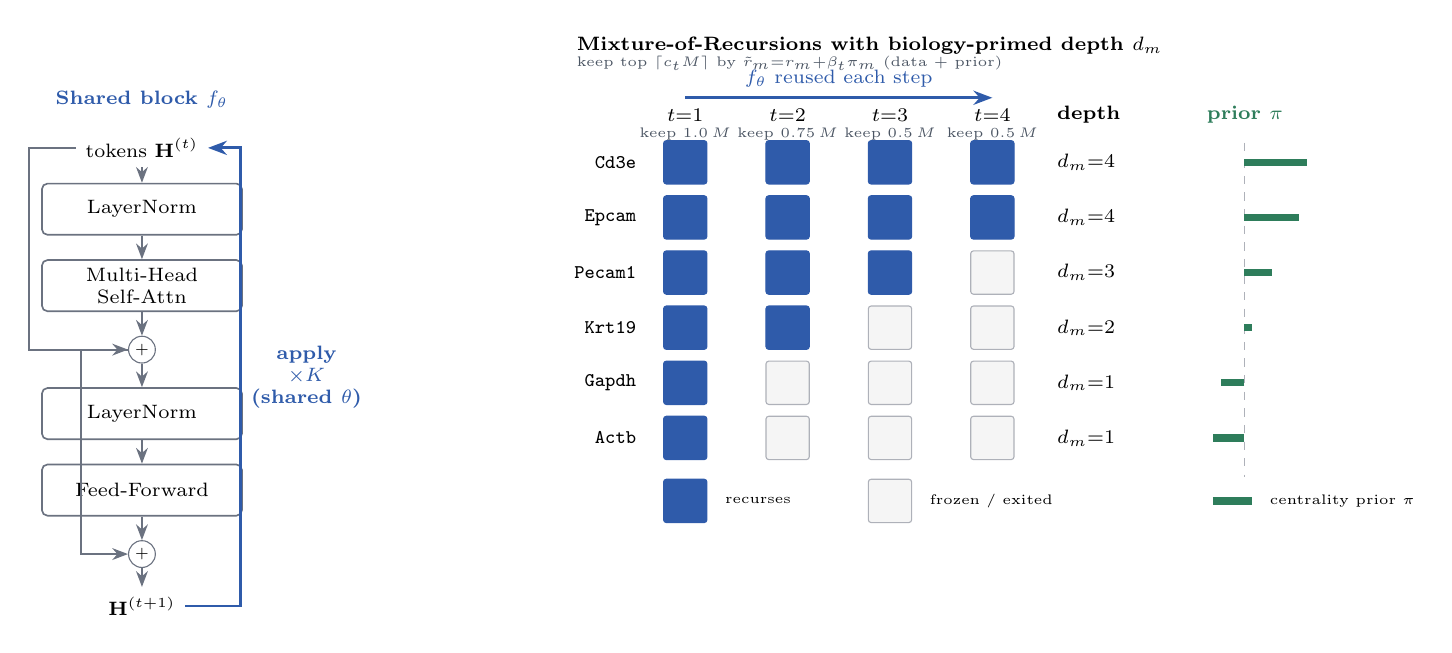
\begin{tikzpicture}[
  font=\footnotesize,
  blk/.style={rounded corners=2pt, draw=boxedge, line width=0.6pt, fill=white,
              text width=24mm, align=center, minimum height=6.5mm, inner sep=2pt, font=\scriptsize},
  add/.style={circle, draw=boxedge, inner sep=0.3pt, minimum size=3.4mm, font=\tiny},
  fl/.style={-{Stealth[length=2mm]}, line width=0.7pt, draw=boxedge},
  rec/.style={-{Stealth[length=2.4mm]}, line width=1.0pt, draw=accentB},
  on/.style={rounded corners=1pt, fill=accentB, draw=accentB, minimum size=5.5mm, inner sep=0pt},
  off/.style={rounded corners=1pt, fill=black!4, draw=boxedge!55, minimum size=5.5mm, inner sep=0pt},
  hd/.style={font=\scriptsize\bfseries},
]
\node[hd, text=accentB] (btitle) {Shared block $f_\theta$};
\node[font=\scriptsize, below=1.4mm of btitle] (bin) {tokens $\mathbf{H}^{(t)}$};
\node[blk, below=2mm of bin] (ln1) {LayerNorm};
\node[blk, below=3mm of ln1] (att) {Multi-Head Self-Attn};
\node[add, below=3mm of att] (a1) {$+$};
\node[blk, below=3mm of a1] (ln2) {LayerNorm};
\node[blk, below=3mm of ln2] (ffn) {Feed-Forward};
\node[add, below=3mm of ffn] (a2) {$+$};
\node[font=\scriptsize, below=2.4mm of a2] (bout) {$\mathbf{H}^{(t{+}1)}$};
\draw[fl] (bin)--(ln1); \draw[fl] (ln1)--(att); \draw[fl] (att)--(a1);
\draw[fl] (a1)--(ln2); \draw[fl] (ln2)--(ffn); \draw[fl] (ffn)--(a2); \draw[fl] (a2)--(bout);
\draw[fl] (bin.west) -- ++(-6mm,0) |- (a1.west);
\draw[fl] (a1.west) -- ++(-6mm,0) |- (a2.west);
\draw[rec] (bout.east) -- ++(7mm,0) |- (bin.east)
   node[pos=0.25, right, align=center, text=accentB, font=\scriptsize\bfseries] {apply\\$\times K$\\(shared $\theta$)};

\begin{scope}[shift={(56mm,-8mm)}]
  \node[hd, anchor=south west] at (-2mm,12.5mm) {Mixture-of-Recursions with biology-primed depth $d_m$};
  \node[font=\tiny, text=subcap, anchor=south west] at (-2mm,10.4mm)
     {keep top $\lceil c_t M\rceil$ by $\tilde r_m{=}r_m{+}\beta_t\pi_m$ (data $+$ prior)};
  \draw[rec] (1*13mm,8.2mm) -- (4*13mm,8.2mm)
     node[midway, above, font=\scriptsize, text=accentB] {$f_\theta$ reused each step};
  \foreach \t/\c in {1/1.0, 2/0.75, 3/0.5, 4/0.5}{
     \node[hd] at (\t*13mm,6mm) {$t{=}\t$};
     \node[font=\tiny, text=subcap] at (\t*13mm,3.6mm) {keep $\c\,M$};
  }
  % genomap centrality prior pi (label-free): a bar per gene, longer = more central
  % hub -> primed to recurse deeper. Visually correlates high pi with deep d_m.
  \node[hd, anchor=west, text=accentA] at (78mm,6mm) {prior $\pi$};
  \draw[boxedge!55, line width=0.4pt, dashed] (84mm,2.5mm) -- (84mm,-6*7mm+2mm);
  \foreach \g/\d/\r/\pp in {Cd3e/4/0/1.6, Epcam/4/1/1.4, Pecam1/3/2/0.7, Krt19/2/3/0.2, Gapdh/1/4/-0.6, Actb/1/5/-0.8}{
     \node[anchor=east, font=\scriptsize\ttfamily] at (8mm,-\r*7mm) {\g};
     \foreach \t in {1,...,4}{
        \ifnum\t>\d \node[off] at (\t*13mm,-\r*7mm) {}; \else \node[on] at (\t*13mm,-\r*7mm) {}; \fi
     }
     \node[anchor=west, font=\scriptsize] at (4*13mm+7mm,-\r*7mm) {$d_m{=}\d$};
     \draw[accentA, line width=2.6pt] (84mm,-\r*7mm) -- ++(\pp*5mm,0);
  }
  \node[hd, anchor=west] at (4*13mm+7mm,6mm) {depth};
  \node[on] (lg1) at (1*13mm,-6*7mm-1mm) {};
  \node[anchor=west, font=\tiny] at ([xshift=1mm]lg1.east) {recurses};
  \node[off] (lg2) at (3*13mm,-6*7mm-1mm) {};
  \node[anchor=west, font=\tiny] at ([xshift=1mm]lg2.east) {frozen / exited};
  \draw[accentA, line width=2.6pt] (80mm,-6*7mm-1mm) -- ++(5mm,0);
  \node[anchor=west, font=\tiny] at (86mm,-6*7mm-1mm) {centrality prior $\pi$};
\end{scope}
\end{tikzpicture}%
}
\caption{\textbf{Biology-informed Mixture-of-Recursions.} \emph{Left:} one
weight-shared pre-norm block $f_\theta$ (the model's only transformer parameters) is
re-applied up to $K{=}4$ times, so depth costs no extra parameters. \emph{Right:} an
expert-choice router keeps a shrinking top fraction of markers per step (capacity
funnel $1,\tfrac34,\tfrac12,\tfrac12$); a marker not kept is frozen, so its
\emph{recursion depth} $d_m$ is the deepest step it survived. The keep decision adds a
label-free genomap co-expression-centrality prior $\beta_t\pi_m$ to each logit
(Eq.~\ref{eq:biorouter}); the \textcolor{accentA}{green bars} show that prior $\pi$
(longer $=$ more central a hub), so lineage and hub genes
(\texttt{Cd3e}, \texttt{Epcam}) are primed to recur deepest while settled
house-keeping genes (\texttt{Gapdh}, \texttt{Actb}) exit at $d_m{=}1$. The bar
heights are illustrative of the centrality ordering, not fitted values. The prior graph
may be \emph{fixed} (shown) or \emph{learned} end-to-end; empirically the learned graph is
the decisive win, while a fixed centrality prior does not beat a random-graph control.}
\label{fig:mor}
\end{figure*}

\section{Dataset Details}
\label{app:data}
We use $8$ genomap single-cell datasets \cite{islam2023cartography} converted to
plain CSV (expression + labels + stratified split) -- Baron, Lung, Muraro, Oesophagus,
Segerstolpe, Spleen, T-cell and Xin -- and $3$ Reactome/P-NET multi-omics
cohorts (prostate, BLCA, STAD) whose fixed Reactome pathway tokens pool mutation,
copy-number and expression channels. Per-dataset sample, feature and class counts are
read directly from the result files and summarised in Table~\ref{tab:datasets}.

\begin{table}[h]
\centering
\resizebox{\columnwidth}{!}{%
\begin{tabular}{llrrr}
\toprule
Dataset & Modality & Samples & Features & Classes \\
\midrule
Baron & single-cell & 8{,}569 & 2{,}000 & 13 \\
Lung & single-cell & 57{,}020 & 1{,}089 & 25 \\
Muraro & single-cell & 2{,}122 & 2{,}000 & 9 \\
Oeso. & single-cell & 87{,}947 & 1{,}089 & 18 \\
Seger. & single-cell & 2{,}127 & 2{,}000 & 11 \\
Spleen & single-cell & 94{,}129 & 1{,}089 & 28 \\
T-cell & single-cell & 24{,}007 & 1{,}089 & 7 \\
Xin & single-cell & 1{,}492 & 2{,}000 & 4 \\
\midrule
Prostate & multi-omics & 1{,}011 & 1{,}223 & 2 \\
BLCA & multi-omics & 404 & 1{,}258 & 2 \\
STAD & multi-omics & 414 & 1{,}258 & 2 \\
\bottomrule
\end{tabular}}
\caption{The 11 datasets used throughout: $8$ genomap single-cell suites
and $3$ Reactome/P-NET multi-omics cohorts. Counts are read directly from the
result files.}
\label{tab:datasets}
\end{table}

\section{Effective-FLOPs Accounting}
\label{app:flops}
The compute numbers report per-sample FLOPs of the recursive transformer stack, the
only component routing changes. One application of the shared block to $a$ tokens costs
$\phi(a)=4a^2 d + 4\,a\,d\,d_{\mathrm{ff}}$; the nominal fixed-depth cost is
$\Phi_{\mathrm{nom}}=K\,\phi(M)$ and the effective cost sums one block over the tokens
active at each step, $\Phi_{\mathrm{eff}}=\sum_{t=1}^{K}\phi(a_t)$, where $a_t$ is the
mean number of markers the expert-choice funnel keeps at step $t$. Gene embedding and
marker selection are $\mathcal{O}(Nd)$, identical across routing modes, and excluded
from this stack-level comparison.

\paragraph{End-to-end accounting.}
For completeness we account for the whole forward pass, not only the stack. Three parts
scale with the full gene count $N$: gene embedding $\Theta(Nd)$; the cross-attention
marker router, whose $M$ queries attend over all $N$ gene keys at
$\Theta(MNd)$; and the optional gene-graph smoother, which at rank $r$ costs
$\Theta(Nr)$ (never the $N^2$ dense form). Everything after marker selection -- the
recursive stack, pooling and head -- scales with the compressed budget $M\ll N$ at
$\Theta(M^2d)$ per pass. So the router's $\Theta(MNd)$ term dominates the $N$-scaling
and is \emph{linear} in $N$ (versus the $\Theta(N^2 d)$ self-attention a full-gene
transformer would pay), while the quadratic cost is paid only on the $M$ markers. The
architecture ablations of Table~\ref{tab:ladder} vary only the stack, so the stack-level
ratios there are the correct comparison for the routing/sharing claims; the router and
embedding terms are shared by every variant. Measured wall-clock and peak-memory
profiling on matched hardware is a straightforward addition we leave to the camera-ready.

\section{Theoretical Foundation of the Router}
\label{app:theory}
This appendix gives the mathematical and biological grounding for bioMoR's
biology-informed router.

\paragraph{Routing as conditional computation.}
The router implements \emph{conditional computation}: a learned policy routes each token
to a token-specific amount of compute, the gating principle of sparsely-gated mixtures
of experts \cite{shazeer2017outrageously}, reused by Mixture-of-Depths
\cite{raposo2024mixture} and Mixture-of-Recursions \cite{bae2025mixture}; the
``experts'' here are recursion \emph{depths} of one shared block, which couples adaptive
computation \cite{graves2016adaptive} to weight sharing.

\paragraph{The differentiable handle.}
The discrete top-$k$ has zero gradient almost everywhere, so bioMoR keeps the soft
probability of the chosen route as a multiplicative \emph{gate} on the block output,
$\mathbf{o}_m=g_m\,f_\theta(\mathbf{h}_m)$ with $g_m=\sigma(\tilde r_m)$. Because $g_m$
is smooth in $\mathbf{w}_r$, the chain
$\mathcal{L}\!\leftarrow\!\mathbf{o}_m\!\leftarrow\!g_m\!\leftarrow\!\mathbf{w}_r$ is
unbroken: the hard choice routes, the soft gate carries the gradient. The biological
prior of Eq.~\eqref{eq:biorouter} is an additive constant in this logit, so it shifts
the decision without breaking this path.

\paragraph{Biological foundation of the prior.}
Two facts from single-cell biology motivate the prior. A small set of \emph{marker}
genes carries most discriminative signal
\cite{ianevski2022fully,franzen2019panglaodb,hu2023cellmarker}, so compute should be
allocated unevenly. And gene co-expression networks are approximately scale-free: a few
high-degree \emph{hub} genes (master regulators) exert outsized influence. We
operationalise ``hub'' as eigenvector centrality on the genomap co-expression graph
$\mathbf{W}$: the leading eigenvector $\mathbf{v}$ of
$\mathbf{W}\mathbf{v}=\lambda\mathbf{v}$ scores each gene by the centrality of its
neighbours, recursively, and we $z$-score it to form $\pi$.

\paragraph{Empirical-Bayes reading.}
Equation~\eqref{eq:biorouter} is a log-linear prior on the routing decision, with
$\beta_t\,\pi_m$ a Gaussian-like prior mean and $\beta_t=\beta_0(1-\text{progress})$ a
shrinkage strength that decays as data evidence accumulates: prior-dominated when the
likelihood is uninformative (early training), data-dominated later.

\paragraph{Leakage safety.}
$\mathbf{W}$ is computed from training-split \emph{expression only}; no cell-type label
enters it. The prior therefore injects network topology, not the answer, which is why a
gene-discovery claim under this prior is not circular, unlike a prior built from curated
cell-type marker lists.

\paragraph{Optional pathway-graph smoothing.}
The additive bias treats genes independently. Co-pathway genes should route coherently,
which one obtains by smoothing the logits over $\mathbf{W}$ with the normalised
Laplacian $\mathbf{L}=\mathbf{I}-\mathbf{D}^{-1/2}\mathbf{W}\mathbf{D}^{-1/2}$,
$\hat{\mathbf{r}}^{(t)}=\tilde{\mathbf{r}}^{(t)}-\gamma\,\mathbf{L}\tilde{\mathbf{r}}^{(t)}$
(graph-Laplacian regularisation): a gene borrows routing strength from its network
neighbours. This is one sparse matrix-vector product per step and adds no transformer
parameters; we expose it as an option and leave its evaluation to future work.

\end{document}
